\documentclass[11pt,]{article}
\usepackage[left=1in,top=1in,right=1in,bottom=1in]{geometry}
\newcommand*{\authorfont}{\fontfamily{phv}\selectfont}
\usepackage[]{mathpazo}


  \usepackage[T1]{fontenc}
  \usepackage[utf8]{inputenc}




\usepackage{abstract}
\renewcommand{\abstractname}{}    % clear the title
\renewcommand{\absnamepos}{empty} % originally center

\renewenvironment{abstract}
 {{%
    \setlength{\leftmargin}{0mm}
    \setlength{\rightmargin}{\leftmargin}%
  }%
  \relax}
 {\endlist}

\makeatletter
\def\@maketitle{%
  \newpage
%  \null
%  \vskip 2em%
%  \begin{center}%
  \let \footnote \thanks
    {\fontsize{18}{20}\selectfont\raggedright  \setlength{\parindent}{0pt} \@title \par}%
}
%\fi
\makeatother




\setcounter{secnumdepth}{0}

\usepackage{longtable,booktabs}

\usepackage{graphicx,grffile}
\makeatletter
\def\maxwidth{\ifdim\Gin@nat@width>\linewidth\linewidth\else\Gin@nat@width\fi}
\def\maxheight{\ifdim\Gin@nat@height>\textheight\textheight\else\Gin@nat@height\fi}
\makeatother
% Scale images if necessary, so that they will not overflow the page
% margins by default, and it is still possible to overwrite the defaults
% using explicit options in \includegraphics[width, height, ...]{}
\setkeys{Gin}{width=\maxwidth,height=\maxheight,keepaspectratio}


\title{Economic impact patterns of COVID-19 on emerging market sovereigns,
January to April 2020 \thanks{We gratefully acknowledge the financial support by the Dockson Chair and
the Center of International Studies at USC. Github repository:
\url{https://github.com/timodaehler/COVID19DEBT}. \textbf{Current
version:} June 28, 2020.}  }



\author{\Large Joshua Aizenman\footnote{\href{mailto:aizenman@usc.edu}{\nolinkurl{aizenman@usc.edu}}}\vspace{0.05in} \newline\normalsize\emph{Dockson Chair in Economics and IR, USC and the NBER}   \and \Large Yothin Jinjarak\footnote{\href{mailto:yothin.jinjarak@vuw.ac.nz}{\nolinkurl{yothin.jinjarak@vuw.ac.nz}}}\vspace{0.05in} \newline\normalsize\emph{School of Economics and Finance, VUW, New Zealand}   \and \Large Timo B. Dähler\footnote{\href{mailto:daehler@usc.edu}{\nolinkurl{daehler@usc.edu}}}\vspace{0.05in} \newline\normalsize\emph{SIR, USC}  }


\date{}

\usepackage{titlesec}

\titleformat*{\section}{\normalsize\bfseries}
\titleformat*{\subsection}{\normalsize\itshape}
\titleformat*{\subsubsection}{\normalsize\itshape}
\titleformat*{\paragraph}{\normalsize\itshape}
\titleformat*{\subparagraph}{\normalsize\itshape}


\usepackage{natbib}
\bibliographystyle{apsr}
\usepackage[strings]{underscore} % protect underscores in most circumstances



\newtheorem{hypothesis}{Hypothesis}
\usepackage{setspace}


% set default figure placement to htbp
\makeatletter
\def\fps@figure{htbp}
\makeatother


% move the hyperref stuff down here, after header-includes, to allow for - \usepackage{hyperref}

\makeatletter
\@ifpackageloaded{hyperref}{}{%
\ifxetex
  \PassOptionsToPackage{hyphens}{url}\usepackage[setpagesize=false, % page size defined by xetex
              unicode=false, % unicode breaks when used with xetex
              xetex]{hyperref}
\else
  \PassOptionsToPackage{hyphens}{url}\usepackage[draft,unicode=true]{hyperref}
\fi
}

\@ifpackageloaded{color}{
    \PassOptionsToPackage{usenames,dvipsnames}{color}
}{%
    \usepackage[usenames,dvipsnames]{color}
}
\makeatother
\hypersetup{breaklinks=true,
            bookmarks=true,
            pdfauthor={Joshua Aizenman\footnote{\href{mailto:aizenman@usc.edu}{\nolinkurl{aizenman@usc.edu}}} (Dockson Chair in Economics and IR, USC and the NBER) and Yothin Jinjarak\footnote{\href{mailto:yothin.jinjarak@vuw.ac.nz}{\nolinkurl{yothin.jinjarak@vuw.ac.nz}}} (School of Economics and Finance, VUW, New Zealand) and Timo B. Dähler\footnote{\href{mailto:daehler@usc.edu}{\nolinkurl{daehler@usc.edu}}} (SIR, USC)},
             pdfkeywords = {COVID-19, emerging markets, sovereign debt},  
            pdftitle={Economic impact patterns of COVID-19 on emerging market sovereigns,
January to April 2020},
            colorlinks=true,
            citecolor=blue,
            urlcolor=blue,
            linkcolor=magenta,
            pdfborder={0 0 0}}
\urlstyle{same}  % don't use monospace font for urls

% Add an option for endnotes. -----


% add tightlist ----------
\providecommand{\tightlist}{%
\setlength{\itemsep}{0pt}\setlength{\parskip}{0pt}}

% add some other packages ----------

% \usepackage{multicol}
% This should regulate where figures float
% See: https://tex.stackexchange.com/questions/2275/keeping-tables-figures-close-to-where-they-are-mentioned
\usepackage[section]{placeins}


\begin{document}
	
% \pagenumbering{arabic}% resets `page` counter to 1 
%
% \maketitle

{% \usefont{T1}{pnc}{m}{n}
\setlength{\parindent}{0pt}
\thispagestyle{plain}
{\fontsize{18}{20}\selectfont\raggedright 
\maketitle  % title \par  

}

{
   \vskip 13.5pt\relax \normalsize\fontsize{11}{12} 
\textbf{\authorfont Joshua Aizenman\footnote{\href{mailto:aizenman@usc.edu}{\nolinkurl{aizenman@usc.edu}}}} \hskip 15pt \emph{\small Dockson Chair in Economics and IR, USC and the NBER}   \par \textbf{\authorfont Yothin Jinjarak\footnote{\href{mailto:yothin.jinjarak@vuw.ac.nz}{\nolinkurl{yothin.jinjarak@vuw.ac.nz}}}} \hskip 15pt \emph{\small School of Economics and Finance, VUW, New Zealand}   \par \textbf{\authorfont Timo B. Dähler\footnote{\href{mailto:daehler@usc.edu}{\nolinkurl{daehler@usc.edu}}}} \hskip 15pt \emph{\small SIR, USC}   

}

}








\begin{abstract}

    \hbox{\vrule height .2pt width 39.14pc}

    \vskip 8.5pt % \small 

\noindent With the global outbreak of COVID-19, many countries initially tried to
contain a further spread of the virus and to change the dynamics of the
pandemic with lockdowns and social distancing measures. This had two
immediate effects; On the one hand, global demand collapsed and lead to
a precipitous drop in the price for oil and other resources. On the
other hand, governments had to mitigate the economic consequences on
individuals which resulted directly from the virus or indirectly from
the government imposed lockdowns, thereby expanding government deficits
and bulking up sovereign debt. In the light of financial fragility of
emerging markets during previous global crises, this paper examines the
economic impact of the COVID-19 pandemic on government finances.
Specifically, this paper traces the cross-country associations between
COVID-19 mortality, economic fundamentals, policy interventions, and
their impact on sovereign spreads. Our results suggest\ldots{}


\vskip 8.5pt \noindent \emph{Keywords}: COVID-19, emerging markets, sovereign debt \par

    \hbox{\vrule height .2pt width 39.14pc}



\end{abstract}


\vskip -8.5pt


 % removetitleabstract

\noindent  

\hypertarget{introduction}{%
\section{Introduction}\label{introduction}}

In many respects, the great financial crisis that began in 2007 was one
of global liquidity. Particularly after the burst of Lehman Brothers on
15. September 2008, unprecedented stresses in global markets drove a
worldwide flight into US dollars. This left global commercial banks high
and dry. Otherwise unable to access the dollar liquidity they
desperately needed to roll over their funding, governments and central
banks engaged in a concerted effort to eschew a meltdown of the global
financial system through unprecedented measures of liquidity provision:
extremely low interest rates, swap lines, and quantitative easing. These
liquidity measures had two soothing effects: On the one hand, stress in
the global banking system was alleviated. On the other hand, low
interest rates meant low funding costs. This enabled governments in both
the developing and developed world to finance deficits and pile up
sovereign debt, be it in their own currency or in US dollars. This
relatively smooth period since the pinnacle of the great financial
crisis ended abruptly with COVID-19.

While initially thought contained in Wuhan, the WHO declared COVID-19 a
global pandemic on March 11, 2020 as many countries had started
reporting exponentially growing case numbers. As a consequence,
governments throughout the world rightly focused on halting the spread
of the coronavirus through lockdowns. However, the foreseeable explosion
in sovereign debt as countries scramble to counter the pandemic's grave
economic consequences as well as the economic fallout generated by
border closures and the interruption of entire global supply chains
caused another worldwide flight into US dollars similar to the great
financial crisis starting in 2007. While in the short run this affects
emerging market sovereigns mostly indirectly through an increase in
spreads, the longer-term consequences could be massive and detrimental.

In this research paper, we examine the economic consequences of the
COVID-19 pandemic for 33 investible emerging markets. Specifically, we
perform an exploratory case study that tries to establish the underlying
factors that drive the risk perception of international investors toward
emerging market sovereigns. In doing so, we try to uncover patterns that
could shine a light on the path ahead for emerging market sovereigns and
to identify countries that will be more or less affected by the pandemic
episode.

The rest of the paper is structured as follows: Section 2 motivates the
focus on emerging market sovereigns by pointing out differences between
the current economic crisis and the great financial crisis and by
outlining the specific weaknesses of emerging markets in the light of
COVID-19. Based on this discussion, section 2 concludes by formulating
hypotheses on the drivers behind the financial fragility of emerging
market sovereigns. Section 3 discusses the data and presents the results
of the exploratory analysis. Section 4 concludes

\hypertarget{emerging-market-sovereign-debt-and-covid-19}{%
\section{Emerging market sovereign debt and
COVID-19}\label{emerging-market-sovereign-debt-and-covid-19}}

\hypertarget{motivation-for-focus}{%
\subsection{Motivation for focus}\label{motivation-for-focus}}

The motivation behind focusing on emerging market sovereigns stems from
the idea that the COVID-19 pandemic could lead to a global shortage of
US dollars similar to the situation in 2007, which could morph into an
emerging market debt crisis. In 2007, financialization had proceeded so
far that there was no pool of reserves anywhere worldwide that was large
enough to backstop the system and only a lender of last resort would do.
Since the IMF never had the lending firepower necessary, only the US
Federal Reserve had that kind of money. Thus, it almost single-handedly
saved the global financial system through the reactivation of
decades-old swap lines and a number of individual liquidity facilities.
However, unlike 2007 the crisis of 2020 may be even bigger for two
reasons. On the one hand, the economic slowdown happens in perfect
global synchronization due the very nature of the virus being a global
pandemic. Thus, all governments try to stimulate at the same time,
therefore competing for the same funding sources. On the other hand,
emerging markets now make up about one-third of global GDP while the US'
share is in a gradual decline, and so is the US' relative capacity for
providing dollar-based assets and liquidity.

\hypertarget{specific-problems-of-emerging-markets}{%
\subsection{Specific problems of emerging
markets}\label{specific-problems-of-emerging-markets}}

Against the backdrop of the potential dollar shortage described above,
emerging economies are bound to face particular obstacles which
developed countries only face to a lesser extent. To varying degrees,
emerging economies must navigate the COVID-19 pandemic amid: * worsening
terms of trade * dwindling remittances * domestic economic and health
vulnerabilities * tightening international credit conditions In what
follows, we first discuss each of these obstacles. Later, we derive
hypotheses from the discussion.

\hypertarget{obstacle-1-worsening-terms-of-trade}{%
\subsubsection{Obstacle 1: worsening terms of
trade}\label{obstacle-1-worsening-terms-of-trade}}

On the international trade side of things, many of the emerging
economies are heavily reliant on the economic well-being of developed
markets. In particular, emerging economies are focused on three types of
exports: oil, tourism, and intermediate goods.

Oil is a central pillar for many emerging economies, either as exports
or as imports (see graph). For oil exporting emerging economies, oil
revenues affect government finances either directly or indirectly. Some
emerging market governments directly own oil producing companies or the
rights to oil exports and thus hurt from lower oil revenues. Other
governments indirectly hurt from lower oil exports as their revenue base
shrinks when oil producing companies report falling revenues and
earnings. For example in Nigeria, the largest economy in Africa, oil
accounts for about 90 percent of exports and two-thirds of government
revenue, two-thirds of which is destined to service debt. Oil importing
countries primarily benefit from lower oil prices.

Export revenues through tourism is another central pillar for many
emerging economies. (See graph). However, due to extensive quarantines
and border-closures, international arrivals dropped precipitously.

The flight to US dollars induced a rapid depreciation of many emerging
market currencies. This in turn leads to an increase in costs of
imports, which hurts the spending power of households which are already
struggling with income losses due to economic lockdowns and reduced
exports. Of course, the depreciation also leads to strains when it comes
to paying back debt in foreign currency. More about this later.

\hypertarget{obstacle-2-dwingdling-remittances}{%
\subsubsection{Obstacle 2: dwingdling
remittances}\label{obstacle-2-dwingdling-remittances}}

In recent years, remittances were on track to become the largest source
of external finance in developing countries, overtaking FDI flows. For
example, excluding China, remittances to LMICs (\$462 billion) were
significantly larger than FDI flows in 2018 (\$344 billion) according to
the World Bank. These annual remittances of around \$500 billion from
nationals working overseas contribute significantly to emerging market
GDP, savings and financing balance of payments. The Philippines, for
example, receives around \$34 billion a year in this manner, reducing
the country's current account deficit from 10\% to around 1.5\% of GDP.
These remittances, which come primarily from foreign workers in
hospitality, domestic work and construction, are bound to decrease as
these are job fields that are particularly affected by the lockdown
measures implemented in developing countries. Lower remittances
ultimately affect the tax base of governments and hence worsens the
outlook for sovereign finances.

\hypertarget{obstacle-3-domestic-economic-and-health-vulnerability}{%
\subsubsection{Obstacle 3: domestic economic and health
vulnerability}\label{obstacle-3-domestic-economic-and-health-vulnerability}}

Alongside the pain felt through reduced exports, worsening terms of
trade, and decreasing remittances, the domestic economy of emerging
markets appears relatively vulnerable to lockdown measures. Compared to
developed countries, emerging economies on average have a larger share
of the labor force employed in very small firms and workers have
relatively low levels of education. These features of emerging economies
increase the direct cost of social distancing because the share of jobs
that can be done at home is much smaller. As such, there is a dire
trade-off: open up and risk long-lasting negative supply shocks and
human misery through countless mortalities but having a shallower
recession and therefore higher tax revenues, or remaining relatively
shut-down but risking a deeper recession, economic misery and therefore
lower tax revenues, and ultimately political unrest. On top of this
trade-off, even a gradual reopening is harder to do without new waves of
infections. This is because policy measures in emerging economies are
less effective in defeating the virus as hygiene conditions are often
precarious in emerging markets due crowded workplaces and difficult
living conditions.

\hypertarget{obstacle-4-tightening-international-credit-conditions}{%
\subsubsection{Obstacle 4: tightening international credit
conditions}\label{obstacle-4-tightening-international-credit-conditions}}

The quick flight to US dollars and the continuing economic uncertainty
render the credit conditions tighter for many emerging economies, both
on the public and the private side. As many emerging market private
corporations as well as sovereigns have borrowed in dollars and their
currencies depreciated quickly, paying back debt will be hard.
Anticipating this, international investors will be hesitant to lend to
emerging market sovereigns, particularly when governments struggle to
credibly commit future tax revenues to pay back debt, which limits their
capacity to refinance outstanding debt. Some emerging market sovereigns
have swap lines with the FED that alleaviate this problem to some
extent. However, there are good reasons to expect the Fed to continue to
be selective in entering swap lines: its goal is not to assist countries
in distress, but rather to ensure that there is sufficient dollar
liquidity to contain an excess increase in dollar strength abroad that
could deepen the contraction at home. This explains the selection of
``systemically important'' emerging economies with deep currency markets
as the choice recipients of the swaps.

In summary, emerging market sovereigns are going through a perfect storm
and how they weather the storm is likely determined by a variety of
factors. The beginning of the crisis has already highlighted existing
divisions between stronger and weaker emerging economies, by putting
governance and economic resilience to the test. South Korea, for
example, has led the world in coronavirus testing and is being hailed as
a model for many Western countries; by keeping track of COVID-19
clusters, it has been able to contain the outbreak without shutting down
its whole economy. Brazil's leadership, by contrast, has invited
criticism by questioning the seriousness of the pandemic despite
infections among senior members of the government. As such, the economic
effects will likely diverge widely. Economies in north Asia, along with
India and Chila, should benefit from lower energy prices; commodity
exporters in Latin America and oil exports in the Middle East and
Central Asia look more exposed.

\hypertarget{hypotheses}{%
\subsection{Hypotheses}\label{hypotheses}}

\begin{itemize}
\tightlist
\item
  \textbf{Hypothesis 1:} Dependence on oil explains financial fragility
  of emerging market sovereigns.
\item
  \textbf{Hypothesis 1a:} Oil exporters more likely to experience spread
  increases
\item
  \textbf{Hypothesis 1b:} Oil importers less likely to experience spread
  increases
\item
  \textbf{Hypothesis 2:} Dependence on remittances likely to influence
  financial fragility of emerging market sovereigns.
\item
  \textbf{Hypothesis 3:} Adaptability of domestic economy likely to
  affect political and economic stability and thus financial fragility
  of emerging market sovereigns.
\item
  \textbf{Hypothesis 4:} Swap lines positive for sovereings.
\end{itemize}

This paper takes stock of the data gathered during the first four to six
months of the year 2020. We say ``four to six'' because at the time of
writing this document (early June), the data for June is not available
yet. However, as soon as that data is available we will rerun the
analysis and see if the results remain stable. In a nutshell: we explain
the change in spread between 12/31/2019 - 04/30/2020 (and 12/31/2019 -
06/30/2020 as soon as the June data is out) through structural,
macroeconomic, and epidemiologic variables.

\hypertarget{defining-the-sample-of-countries}{%
\subsection{Defining the sample of
countries}\label{defining-the-sample-of-countries}}

In a first step, we had to choose which emerging markets we want to
investigate. Since we are interested in the effect of COVID-19 on
governments' ability to finance deficits in a sustainable way--that is,
without increasing spreads beyond reasonable levels--we are primarily
intersted in emerging markets which are ``investible''. As a starting
point, we defined a country's ``investibility'' as being a constituent
of the JPMorgan EMBI (Emerging Market Bond Index). This index gives
investors exposure to U.S. dollar-denominated government bonds issued by
emerging market countries. The index comprises more than 30 emerging
market countries in a single fund. Specifically, when we looked up the
constituent countries of the fund, it appears as if 31 countries are in
the index as of 25 April 2020 (cf.
\href{www.ishares.com/us/products/239572/ishares-jp-morgan-usd-emerging-markets-bond-etf}{https://www.ishares.com/us/products/239572/ishares-jp-morgan-usd-emerging-markets-bond-etf}
). However, some relatively large and potentially important countries
were not represented in the EMBI so that we added India and Thailand to
the sample. This results in a sample of 33 countries. We call it the
``EMBI+2'' sample. This stands in contrast to the other project we are
working on that looks at data of a 155 countries and which we call the
``extended'' sample. See the graph and table below for an overview of
the countries in the sample.

\begin{figure}
\centering
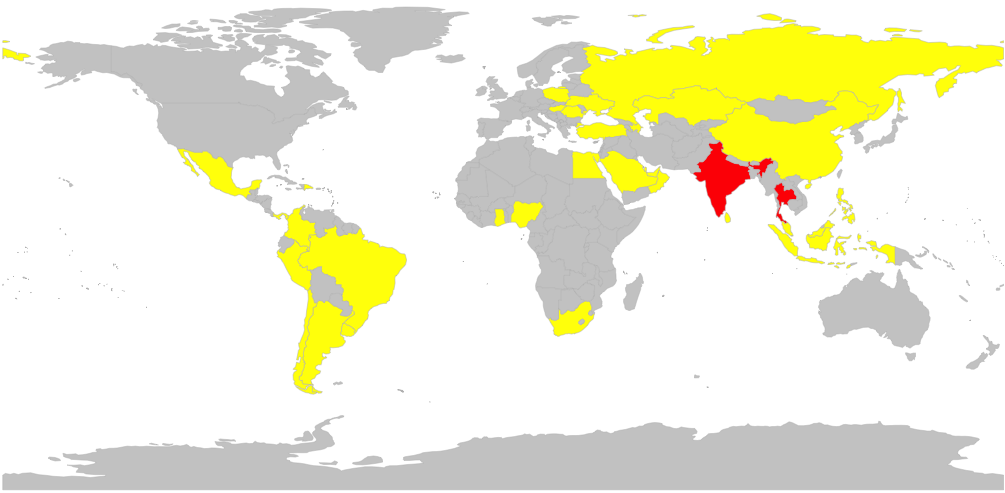
\includegraphics{reportfigures/EMBI+2.png}
\caption{EMBI+2 (Thailand \& India)}
\end{figure}

\begin{longtable}[]{@{}ll@{}}
\toprule
Country & JPM EMBI constituent (1 = yes)\tabularnewline
\midrule
\endhead
Content Cell & Content Cell\tabularnewline
Argentina & 1\tabularnewline
Azerbaijan & 1\tabularnewline
Bahrain & 1\tabularnewline
Brazil & 1\tabularnewline
Chile & 1\tabularnewline
China & 1\tabularnewline
Colombia & 1\tabularnewline
Dominican Republic & 1\tabularnewline
Egypt & 1\tabularnewline
Ghana & 1\tabularnewline
Hungary & 1\tabularnewline
India & 0\tabularnewline
Indonesia & 1\tabularnewline
Kazakhstan & 1\tabularnewline
Malaysia & 1\tabularnewline
Mexico & 1\tabularnewline
Nigeria & 1\tabularnewline
Oman & 1\tabularnewline
Panama & 1\tabularnewline
Peru & 1\tabularnewline
Philippines & 1\tabularnewline
Poland & 1\tabularnewline
Qatar & 1\tabularnewline
Romania & 1\tabularnewline
Russian Federation & 1\tabularnewline
Saudi Arabia & 1\tabularnewline
South Africa & 1\tabularnewline
Sri Lanka & 1\tabularnewline
Thailand & 0\tabularnewline
Turkey & 1\tabularnewline
Ukraine & 1\tabularnewline
United Arab Emirates & 1\tabularnewline
Uruguay & 1\tabularnewline
\bottomrule
\end{longtable}

In addition, we wanted to make sure that all the countris in the sample
are not only investable by being in the EMBI but that they also have a
certain amount of debt outstanding. To that end, we inspected the
Debt/GDP ratio of all EMBI+2 countries in the IMF's global debt database
and checked if all countries have at least a ratio of 20\%. This was
indeed the case so that we didn't drop any of the countries out of the
sample.

The rest of this document is structured as follows: The second part
outlines the data used for the analysis. The third part shows
preliminary results of correlations between the variables. The fourth
part shows regression results and graphical analyses. Part 5 concludes.

\hypertarget{data}{%
\section{2. Data}\label{data}}

In the second step, we obtained data for the outcome variable(s) and the
explanatory variables.

\hypertarget{outcome-variables}{%
\subsection{Outcome variable(s)}\label{outcome-variables}}

\begin{itemize}
\tightlist
\item
  the spread of such bonds over 1-year US treasuries
\item
  the yield of 1-year U.S. dollar-denominated bonds
\item
  the exchange rate vis-à-vis the U.S. dollar
\item
  CDS Specifically, our outcome variables are the changes of these four
  variables between the end of December 2019 and the end of April 2020
  (June 2020). While our main outcome variable of interest is the change
  in spread over U.S. bonds over 4/6 months, we also look at the other
  variables as a robustness check.
\end{itemize}

\begin{figure}
\centering
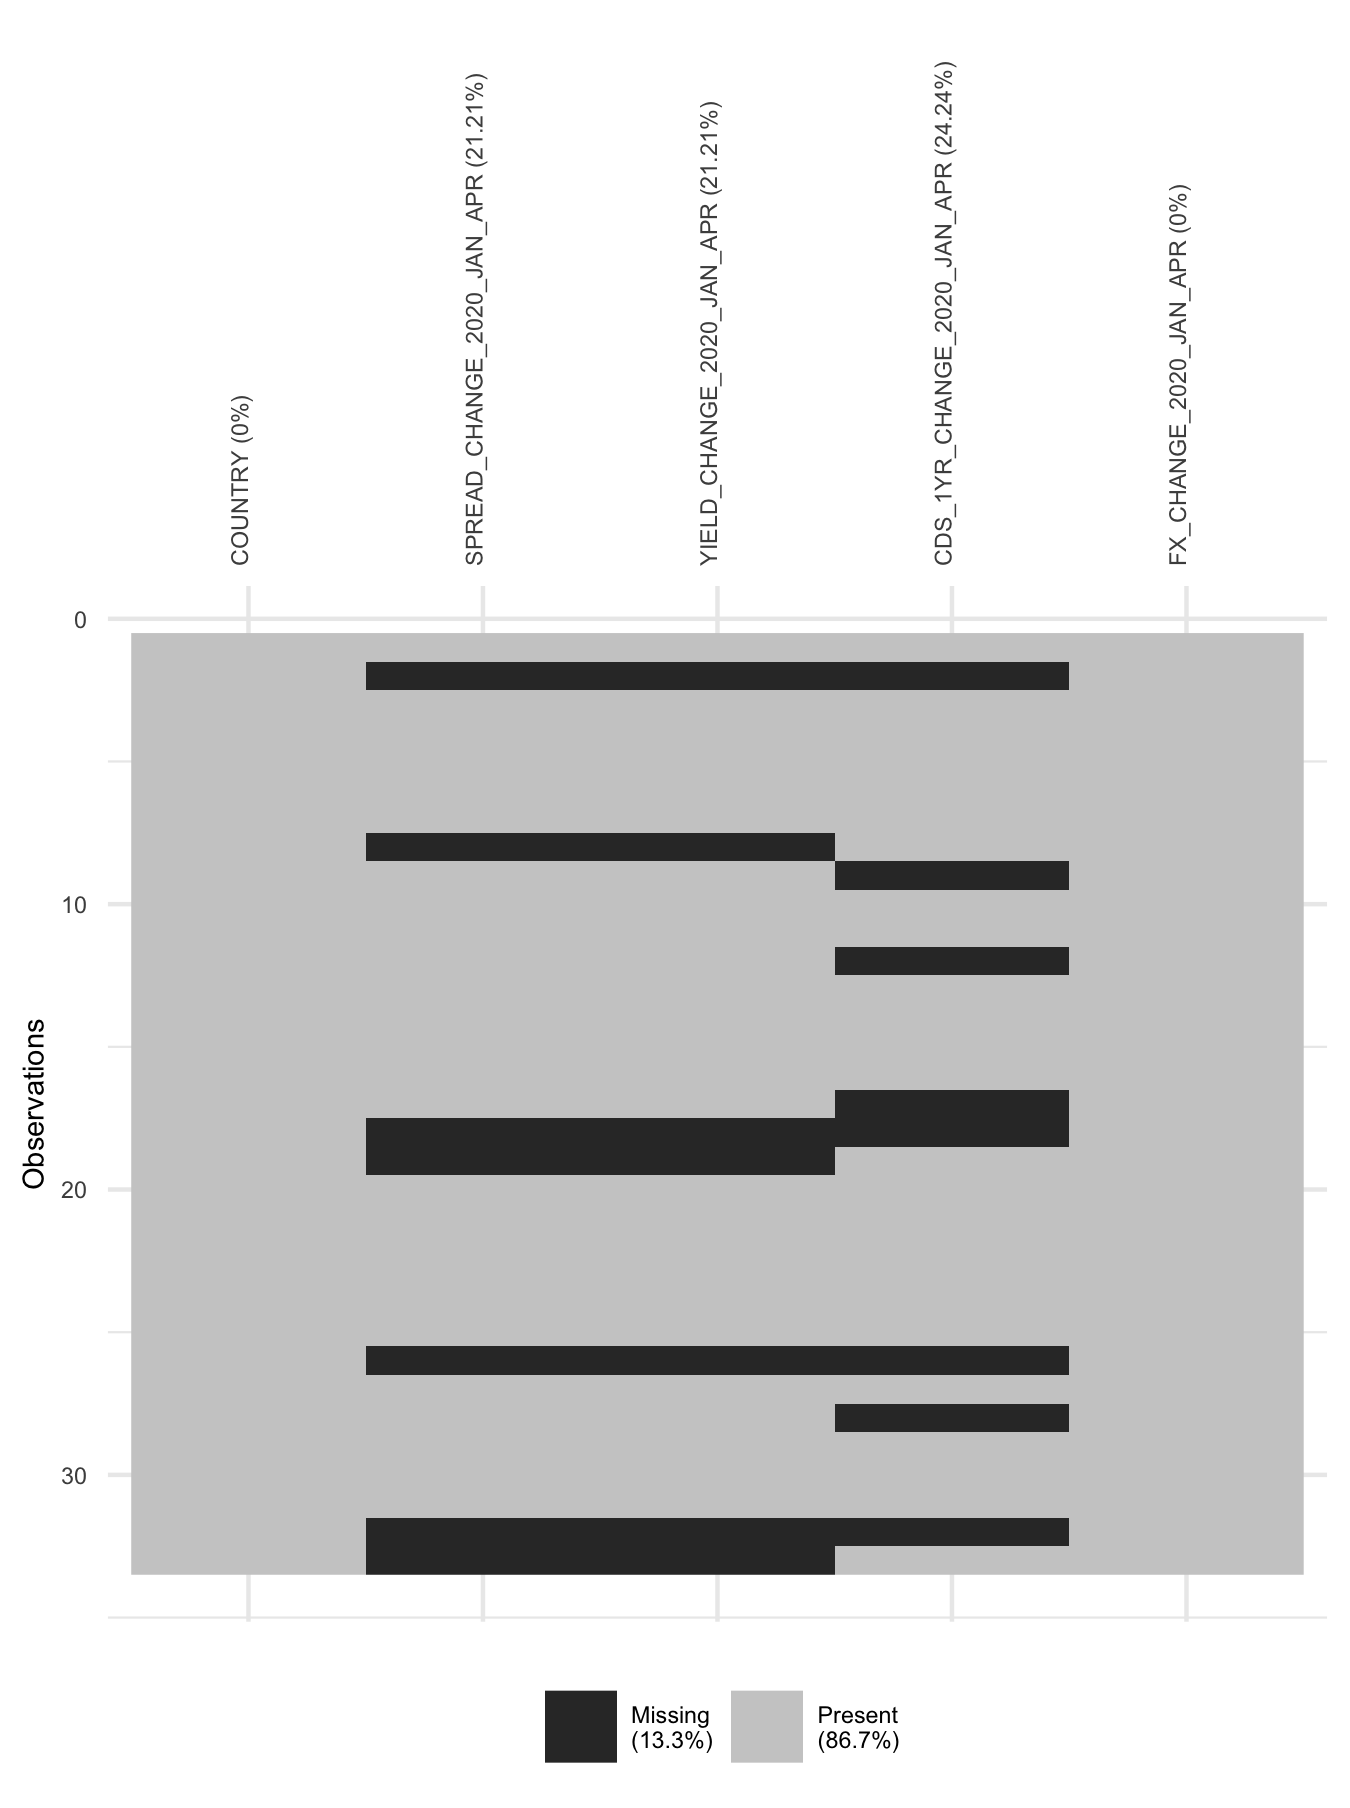
\includegraphics[width=0.5\textwidth,height=\textheight]{reportfigures/missingdata_dependentvariable.png}
\caption{Data availability for dependent variables}
\end{figure}

\hypertarget{explanatory-variables}{%
\subsection{Explanatory variable(s)}\label{explanatory-variables}}

There are a host of explanatory variables in the dataset. Many of them
are diretly sourced from the IMF World Datamapper or from the World
Bank. However, due to the recency of the period of analysis and the lack
of officially published data, we had to hand-code a decent chunk of the
data. To do so, we looked at the IMF's country by country summary of
policy responses to COVID-19
\url{https://www.imf.org/en/Topics/imf-and-covid19/Policy-Responses-to-COVID-19}.
While the following graph does not depict all explanatory variables that
are in the dataset, it does show the most important ones which we also
expect to be the ones that show a clearn pattern in explaning the
economic fragility of emerging markets.

\begin{figure}
\centering
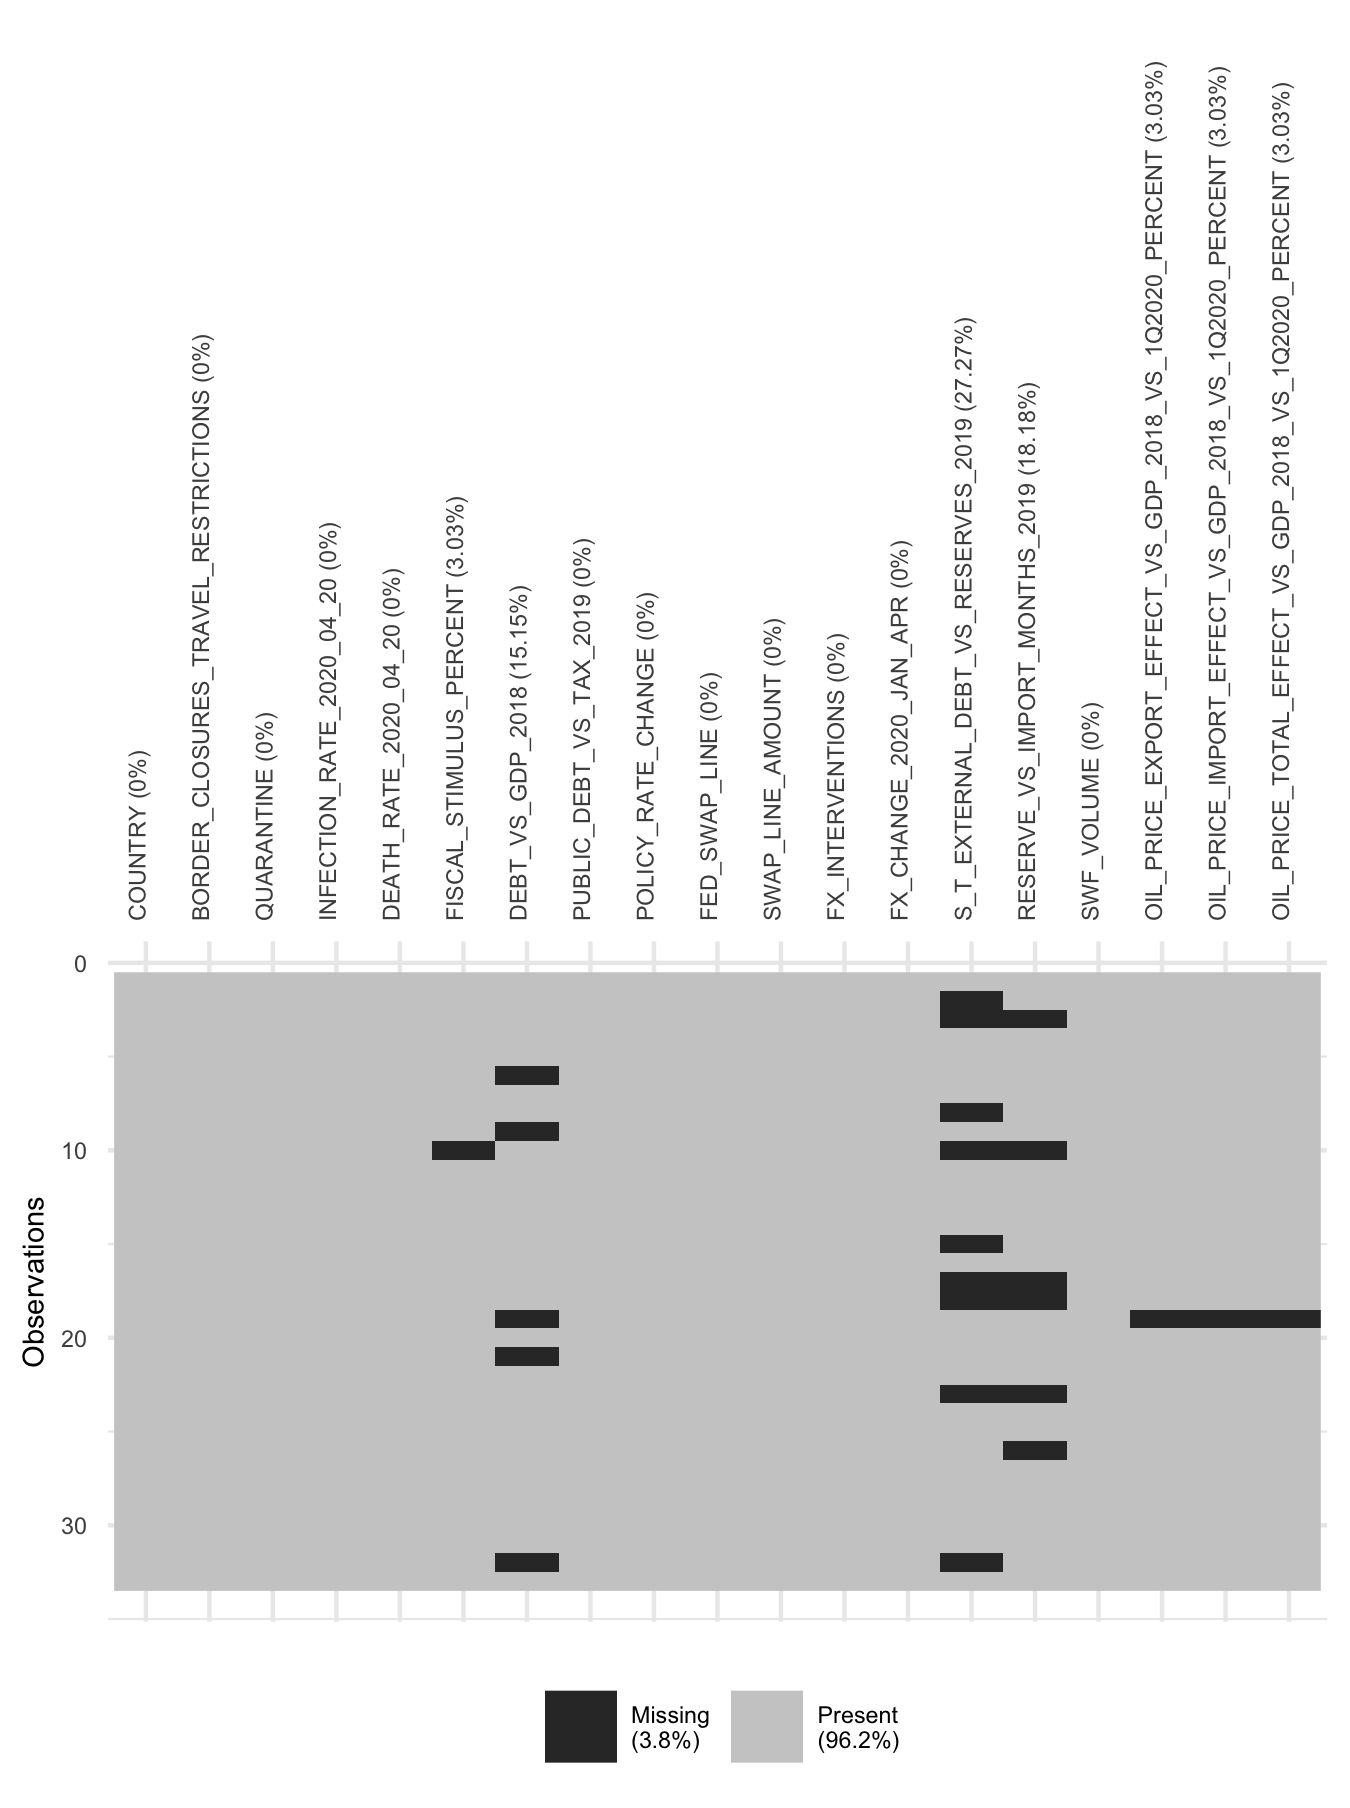
\includegraphics[width=0.5\textwidth,height=\textheight]{reportfigures/missingdata_predictors.png}
\caption{Data availability for explantory variables}
\end{figure}

\hypertarget{data-source}{%
\subsection{Data source}\label{data-source}}

For the specific details on the variable definitions, the sources for
each variable, as well as units and further information, see the sheet
``codebook'' in the document ``data.xlsx''.

\hypertarget{preliminary-patterns-and-correlations}{%
\section{3. Preliminary patterns and
correlations}\label{preliminary-patterns-and-correlations}}

Our dataset comprises more than 100 potential explanatory variables.
However, most of them are not of direct interest and are instead only
used to calculate variables that we use in our regressions. For example,
while both the population size and the mortality is in the dataset, what
is ultimately interesting is the standardized mortality rate per 100,000
people. As such, we do not show correlation matrices of all potential
explantory variables but focus instead on variables that could be used
in the regressions. For ease of overview, we devide the respective
explanatory variables into four clusters:

\begin{itemize}
\tightlist
\item
  Variables related to the pandemic such as whether a quarantine is in
  place, infection rates, mortality rates etc.
\item
  Variables related to fiscal fitness of sovereigns such as debt ratios,
  reserves etc.
\item
  Variables related to monetary aspects such as whether a sovereign has
  a swap line etc.
\item
  Variables related to the effect of oil dependence of a sovereign such
  as the oil share of exports etc.
\end{itemize}

\hypertarget{correlation-matrices}{%
\subsection{Correlation matrices}\label{correlation-matrices}}

\begin{figure}
\centering
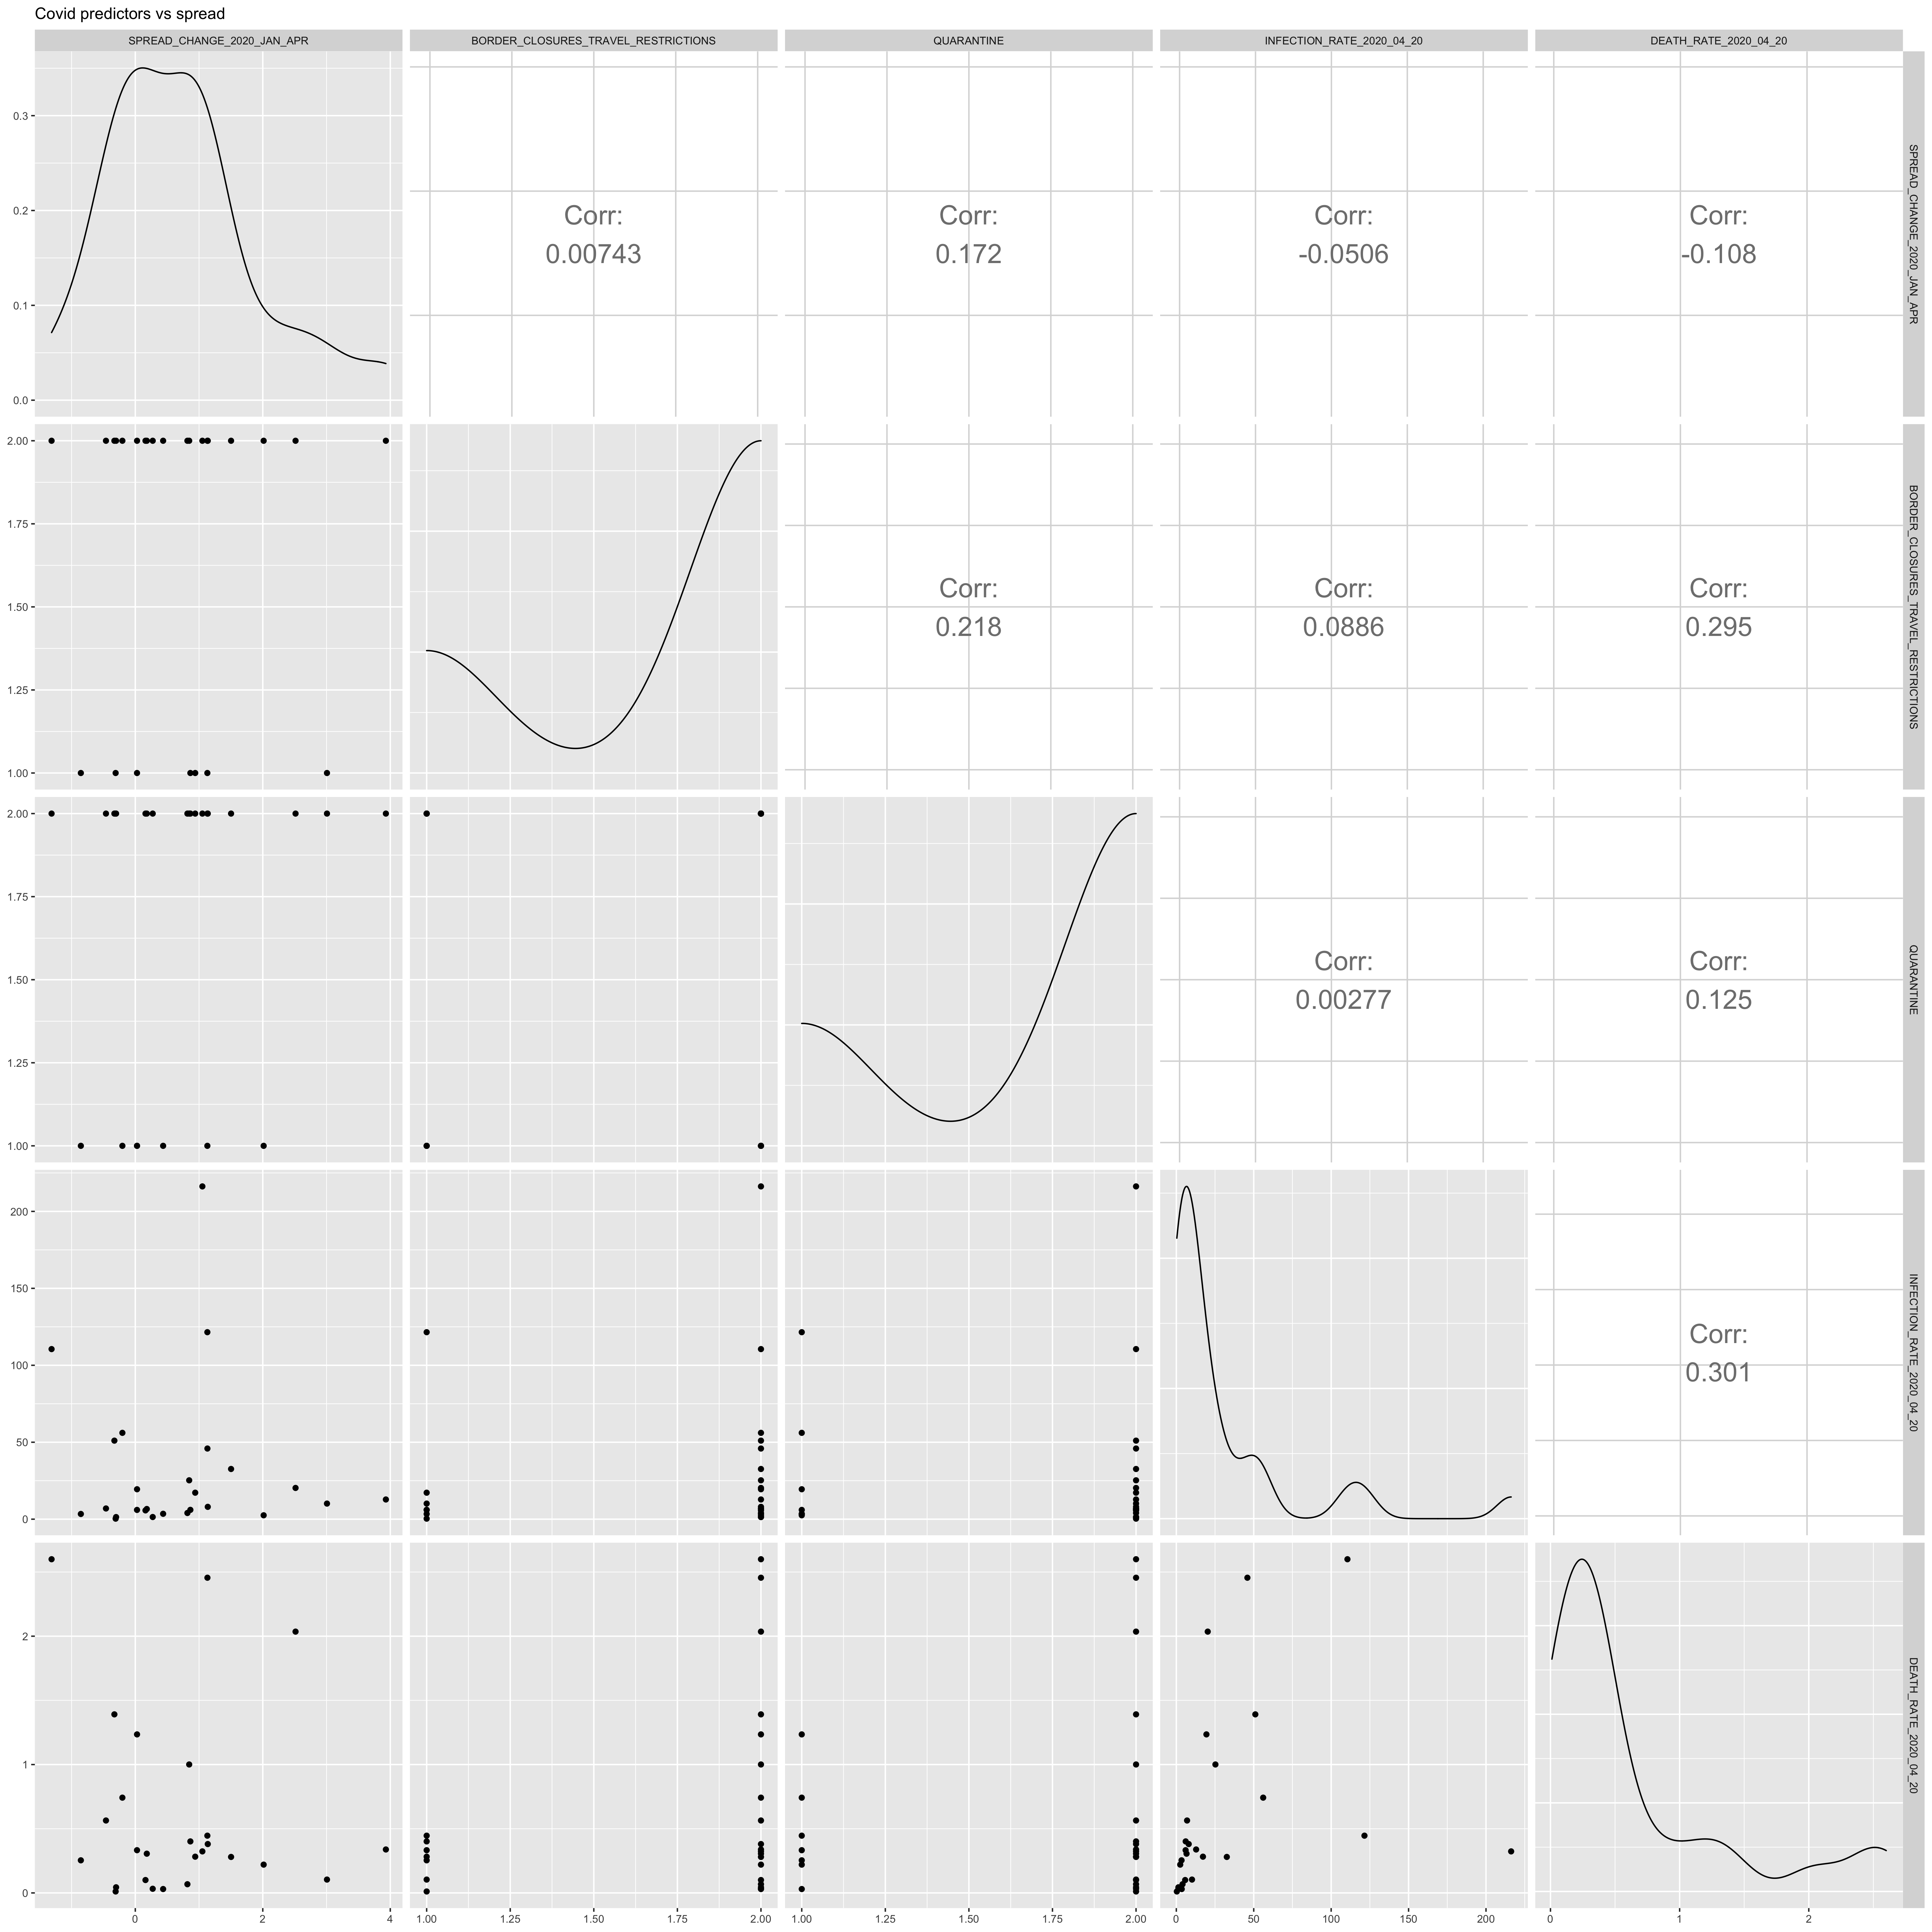
\includegraphics[width=0.5\textwidth,height=\textheight]{reportfigures/Corrmatrix_spread_vs_covid.png}
\caption{Correlation matrix of spread vs explantory variables from the
epidemiologic cluster}
\end{figure}

\begin{figure}
\centering
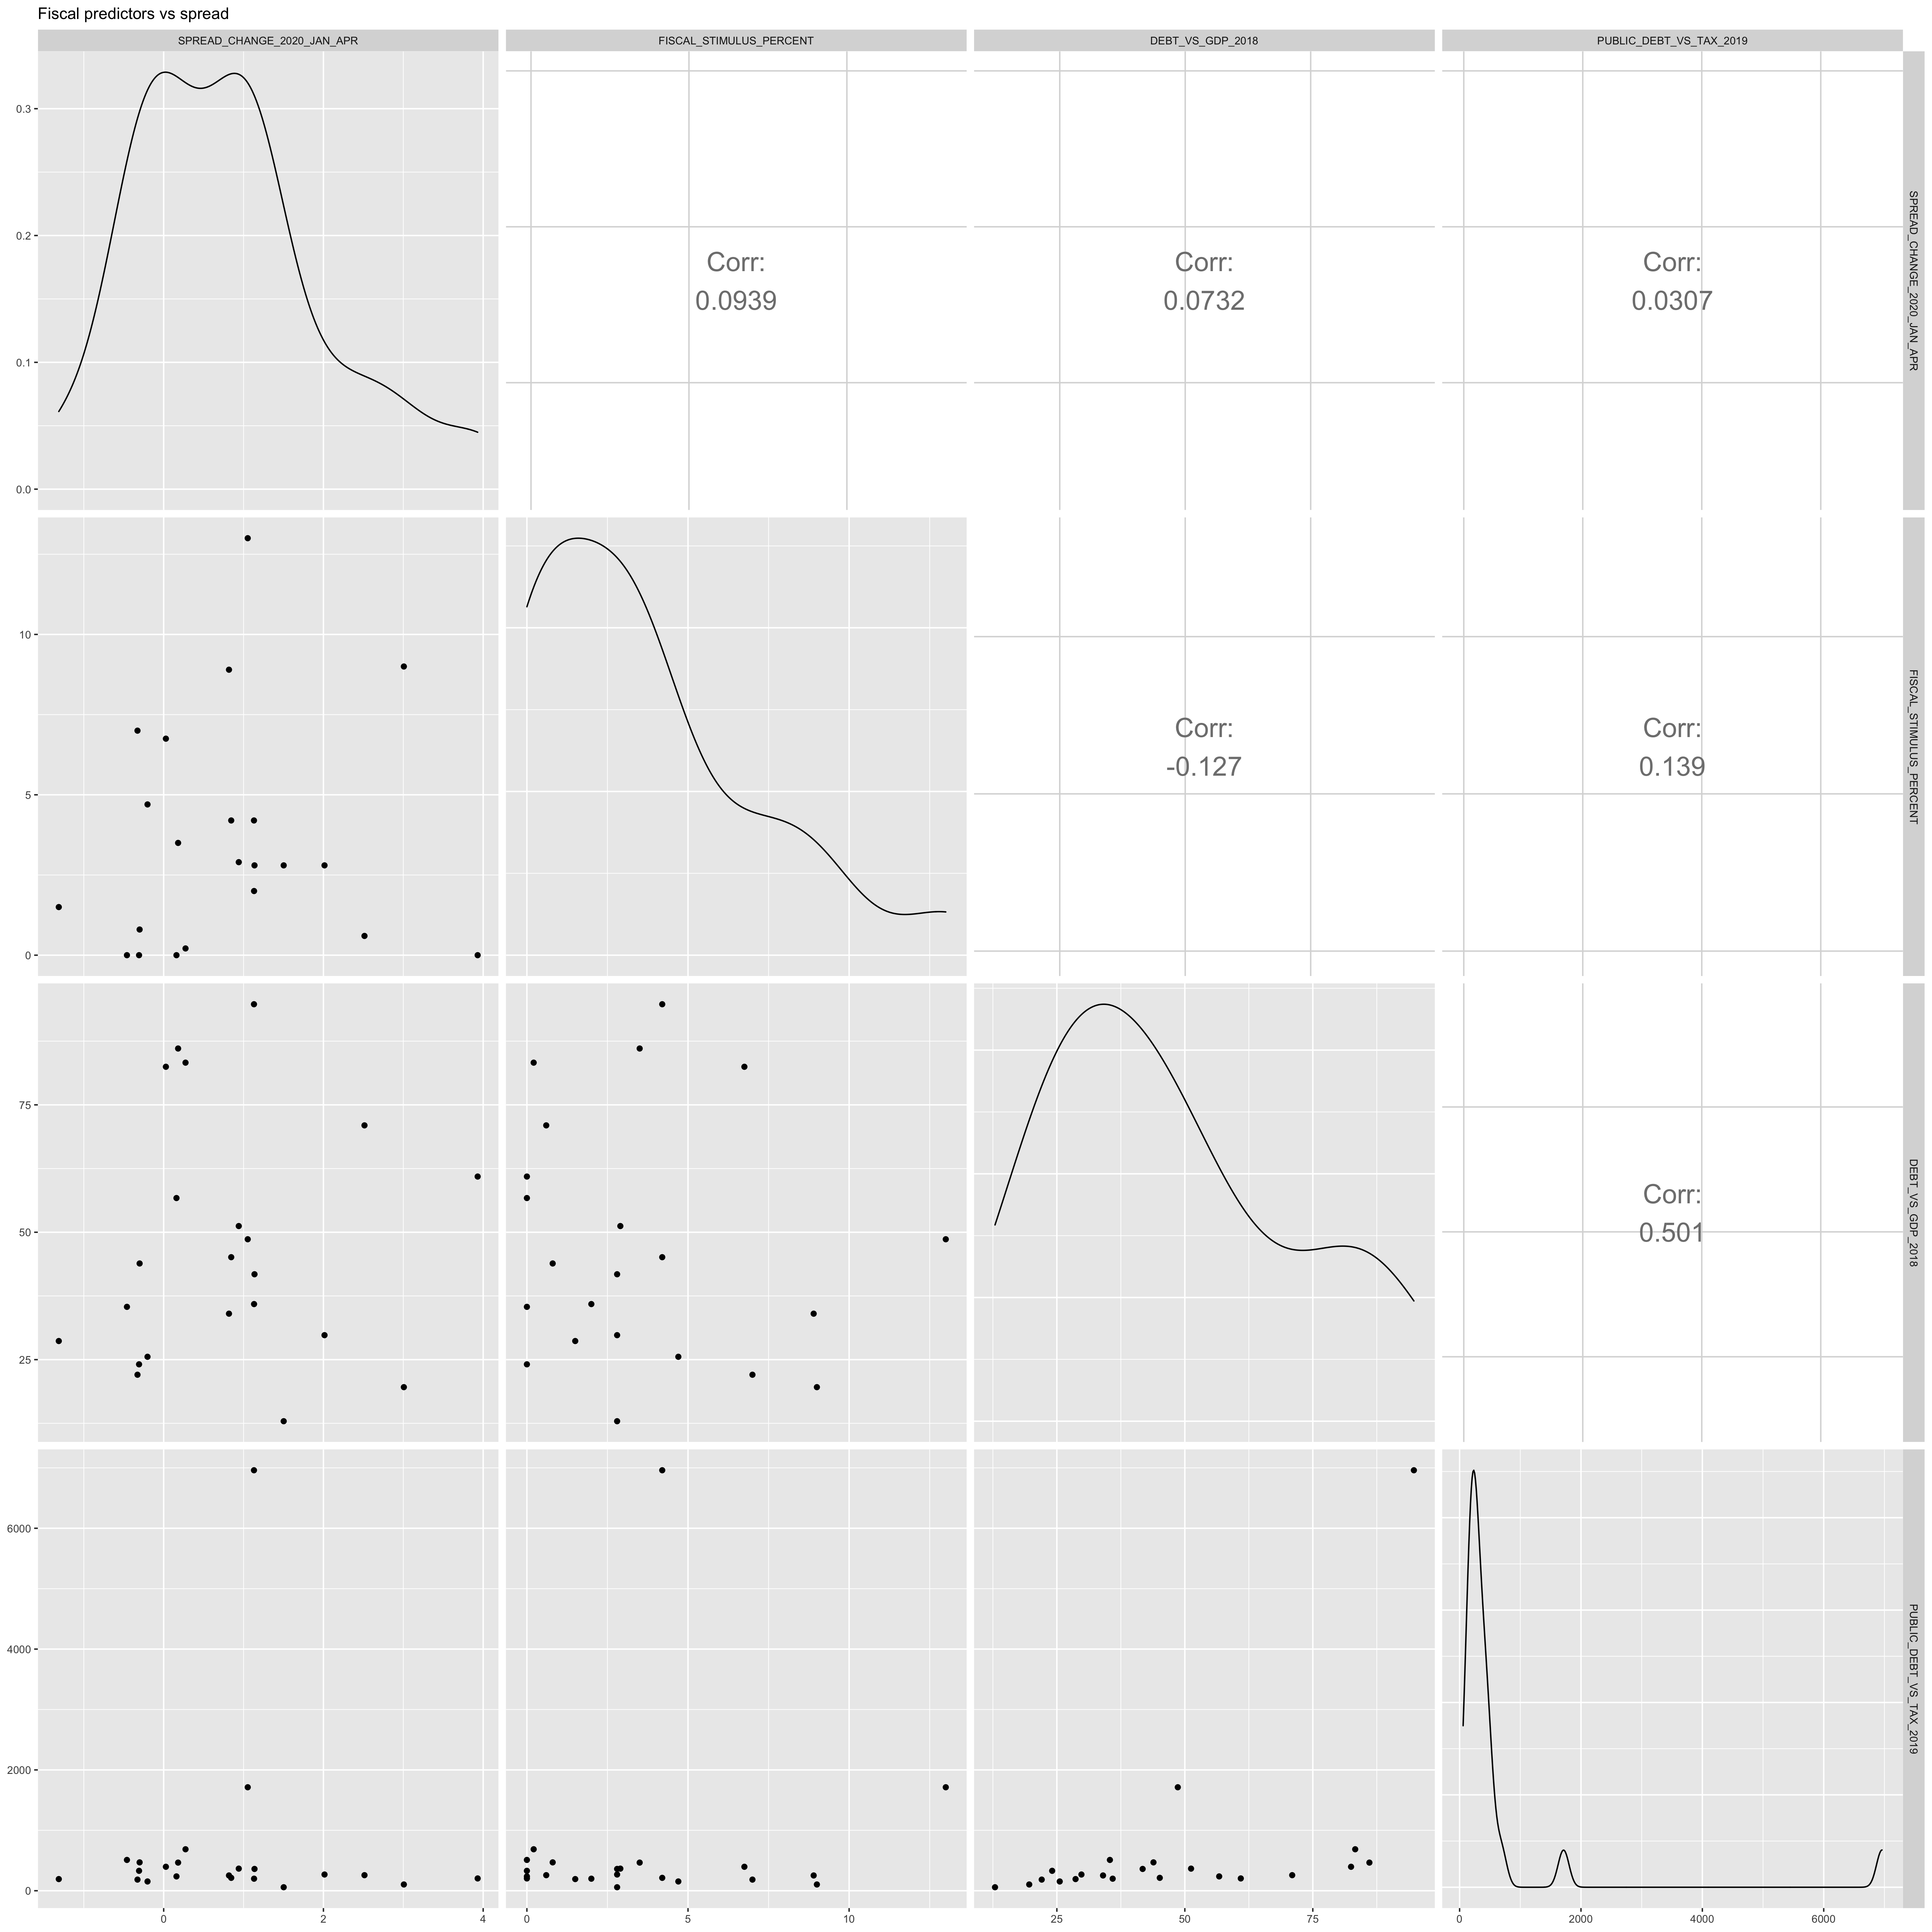
\includegraphics[width=0.5\textwidth,height=\textheight]{reportfigures/Corrmatrix_spread_vs_fiscal.png}
\caption{Correlation matrix of spread vs explantory variables from the
fiscal cluster}
\end{figure}

\begin{figure}
\centering
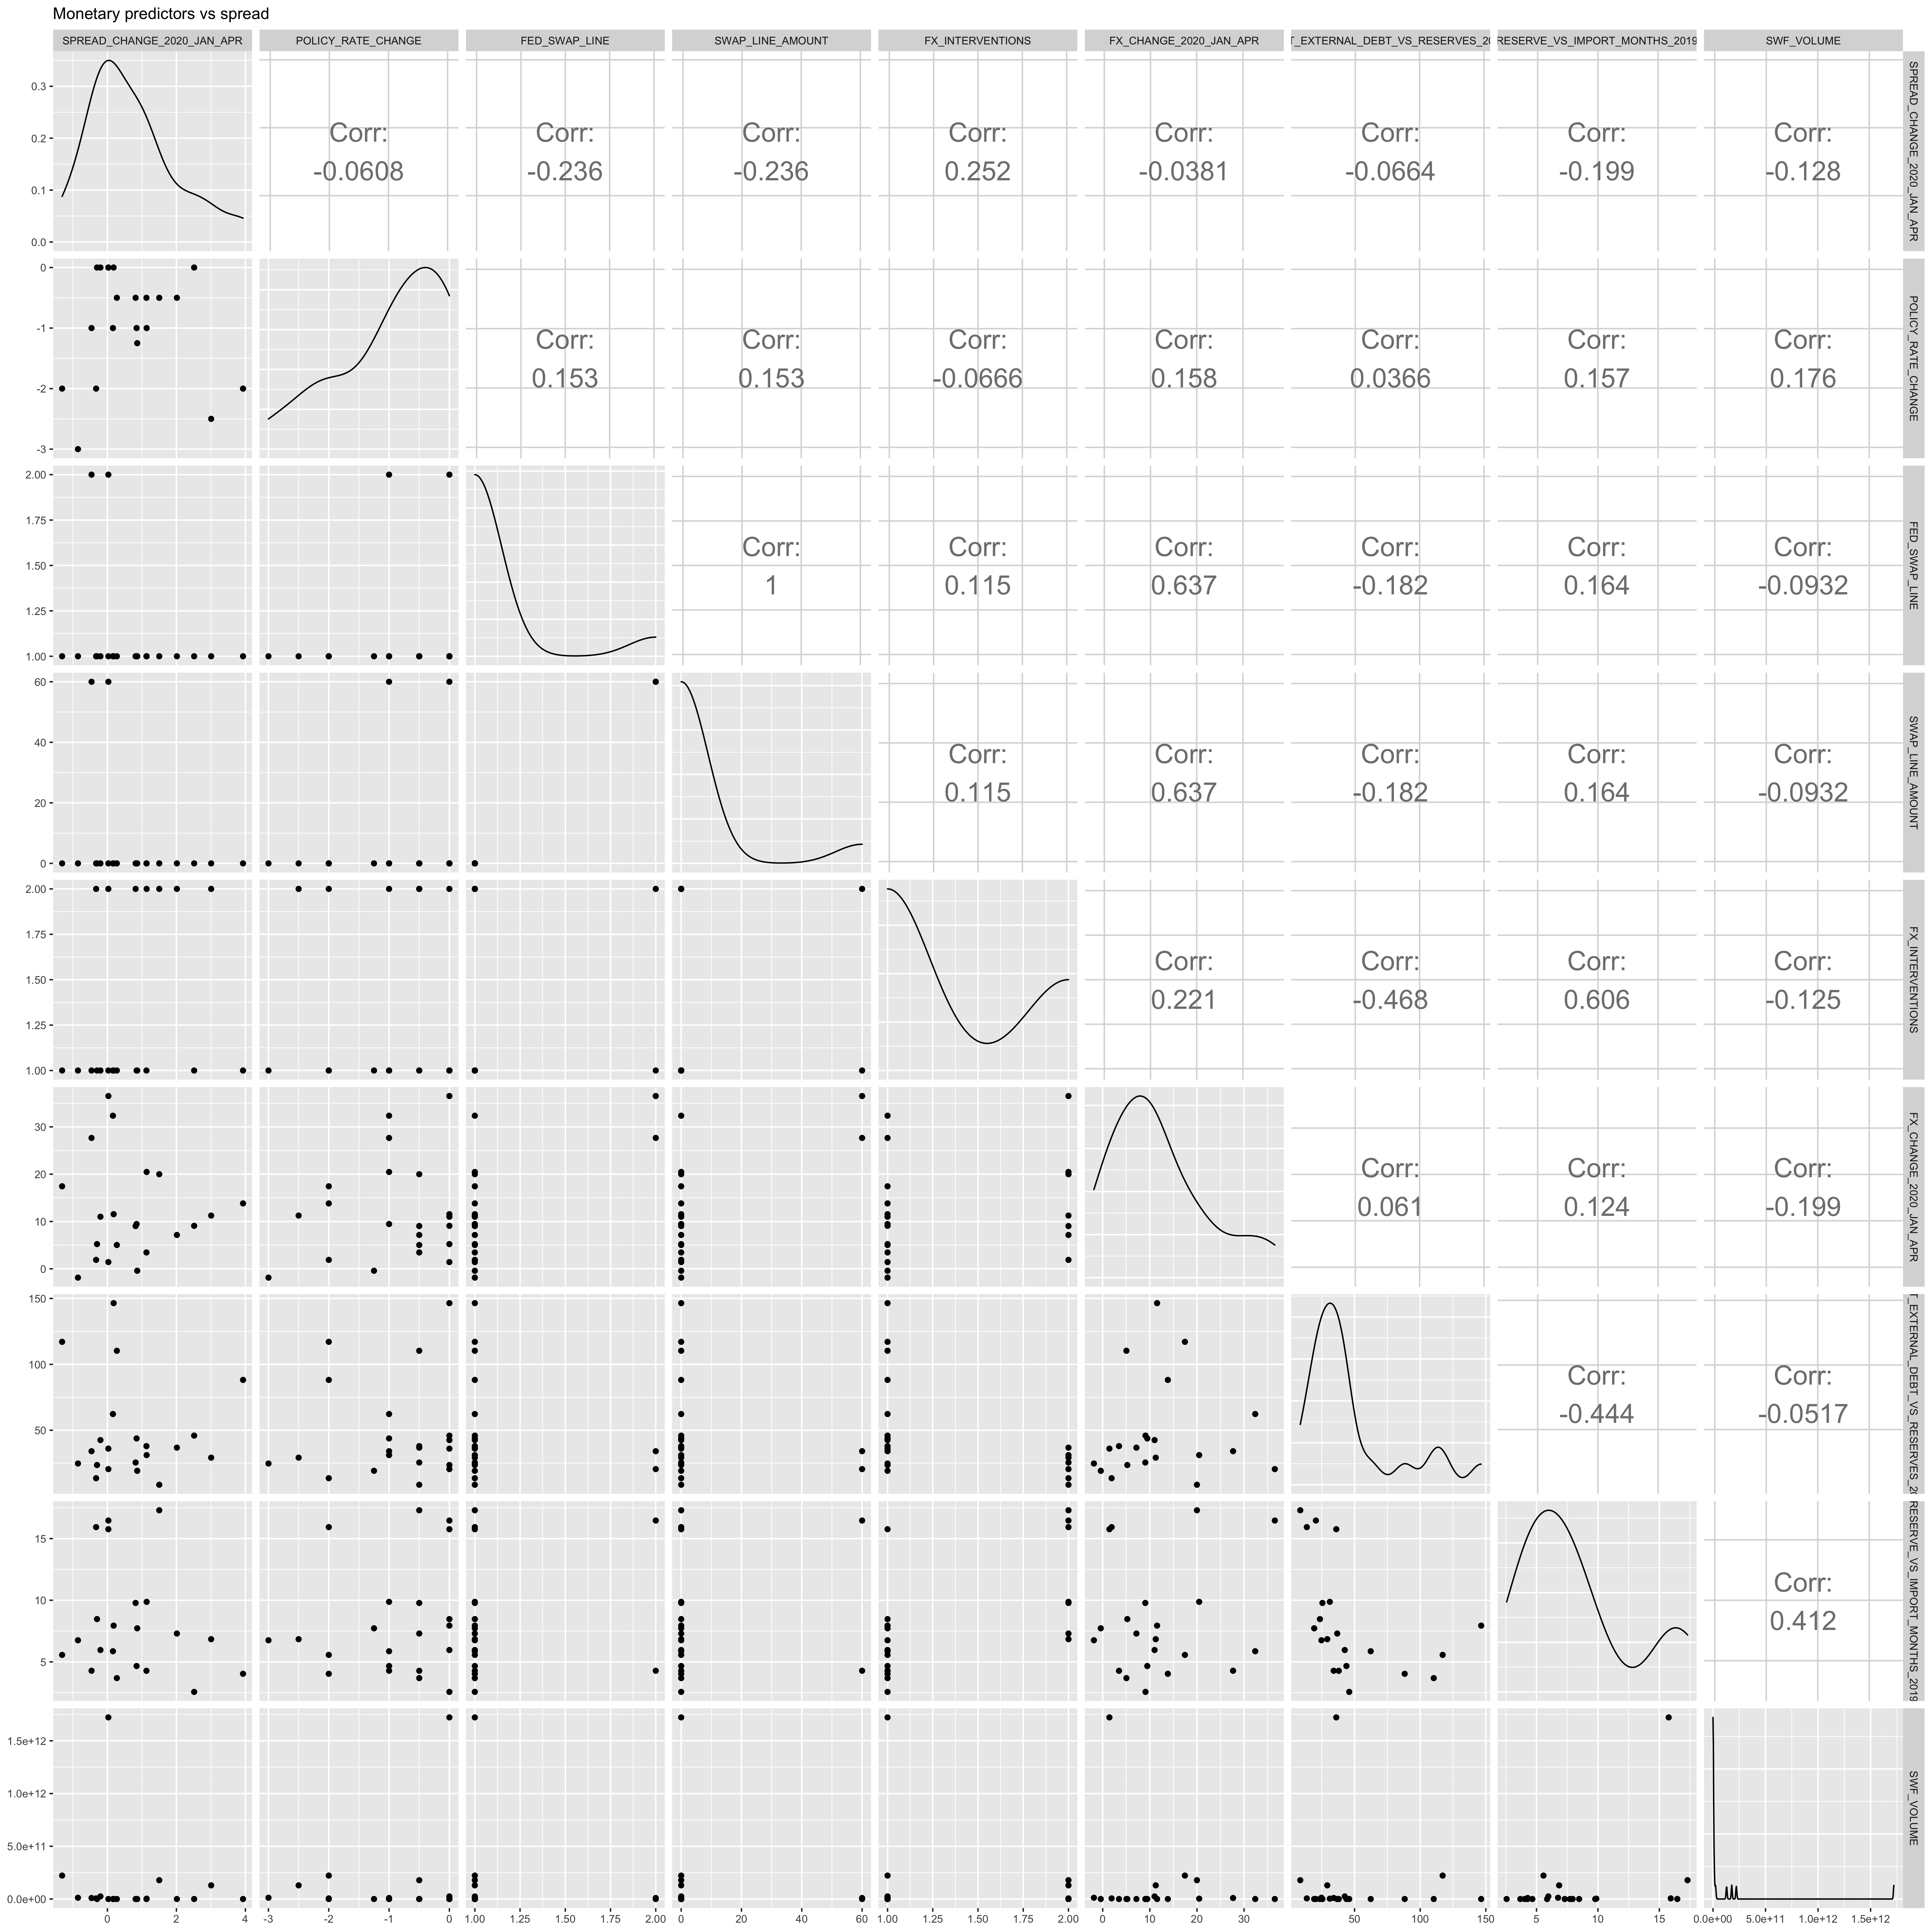
\includegraphics[width=0.5\textwidth,height=\textheight]{reportfigures/Corrmatrix_spread_vs_monetary.png}
\caption{Correlation matrix of spread vs explantory variables from the
monetary cluster}
\end{figure}

\begin{figure}
\centering
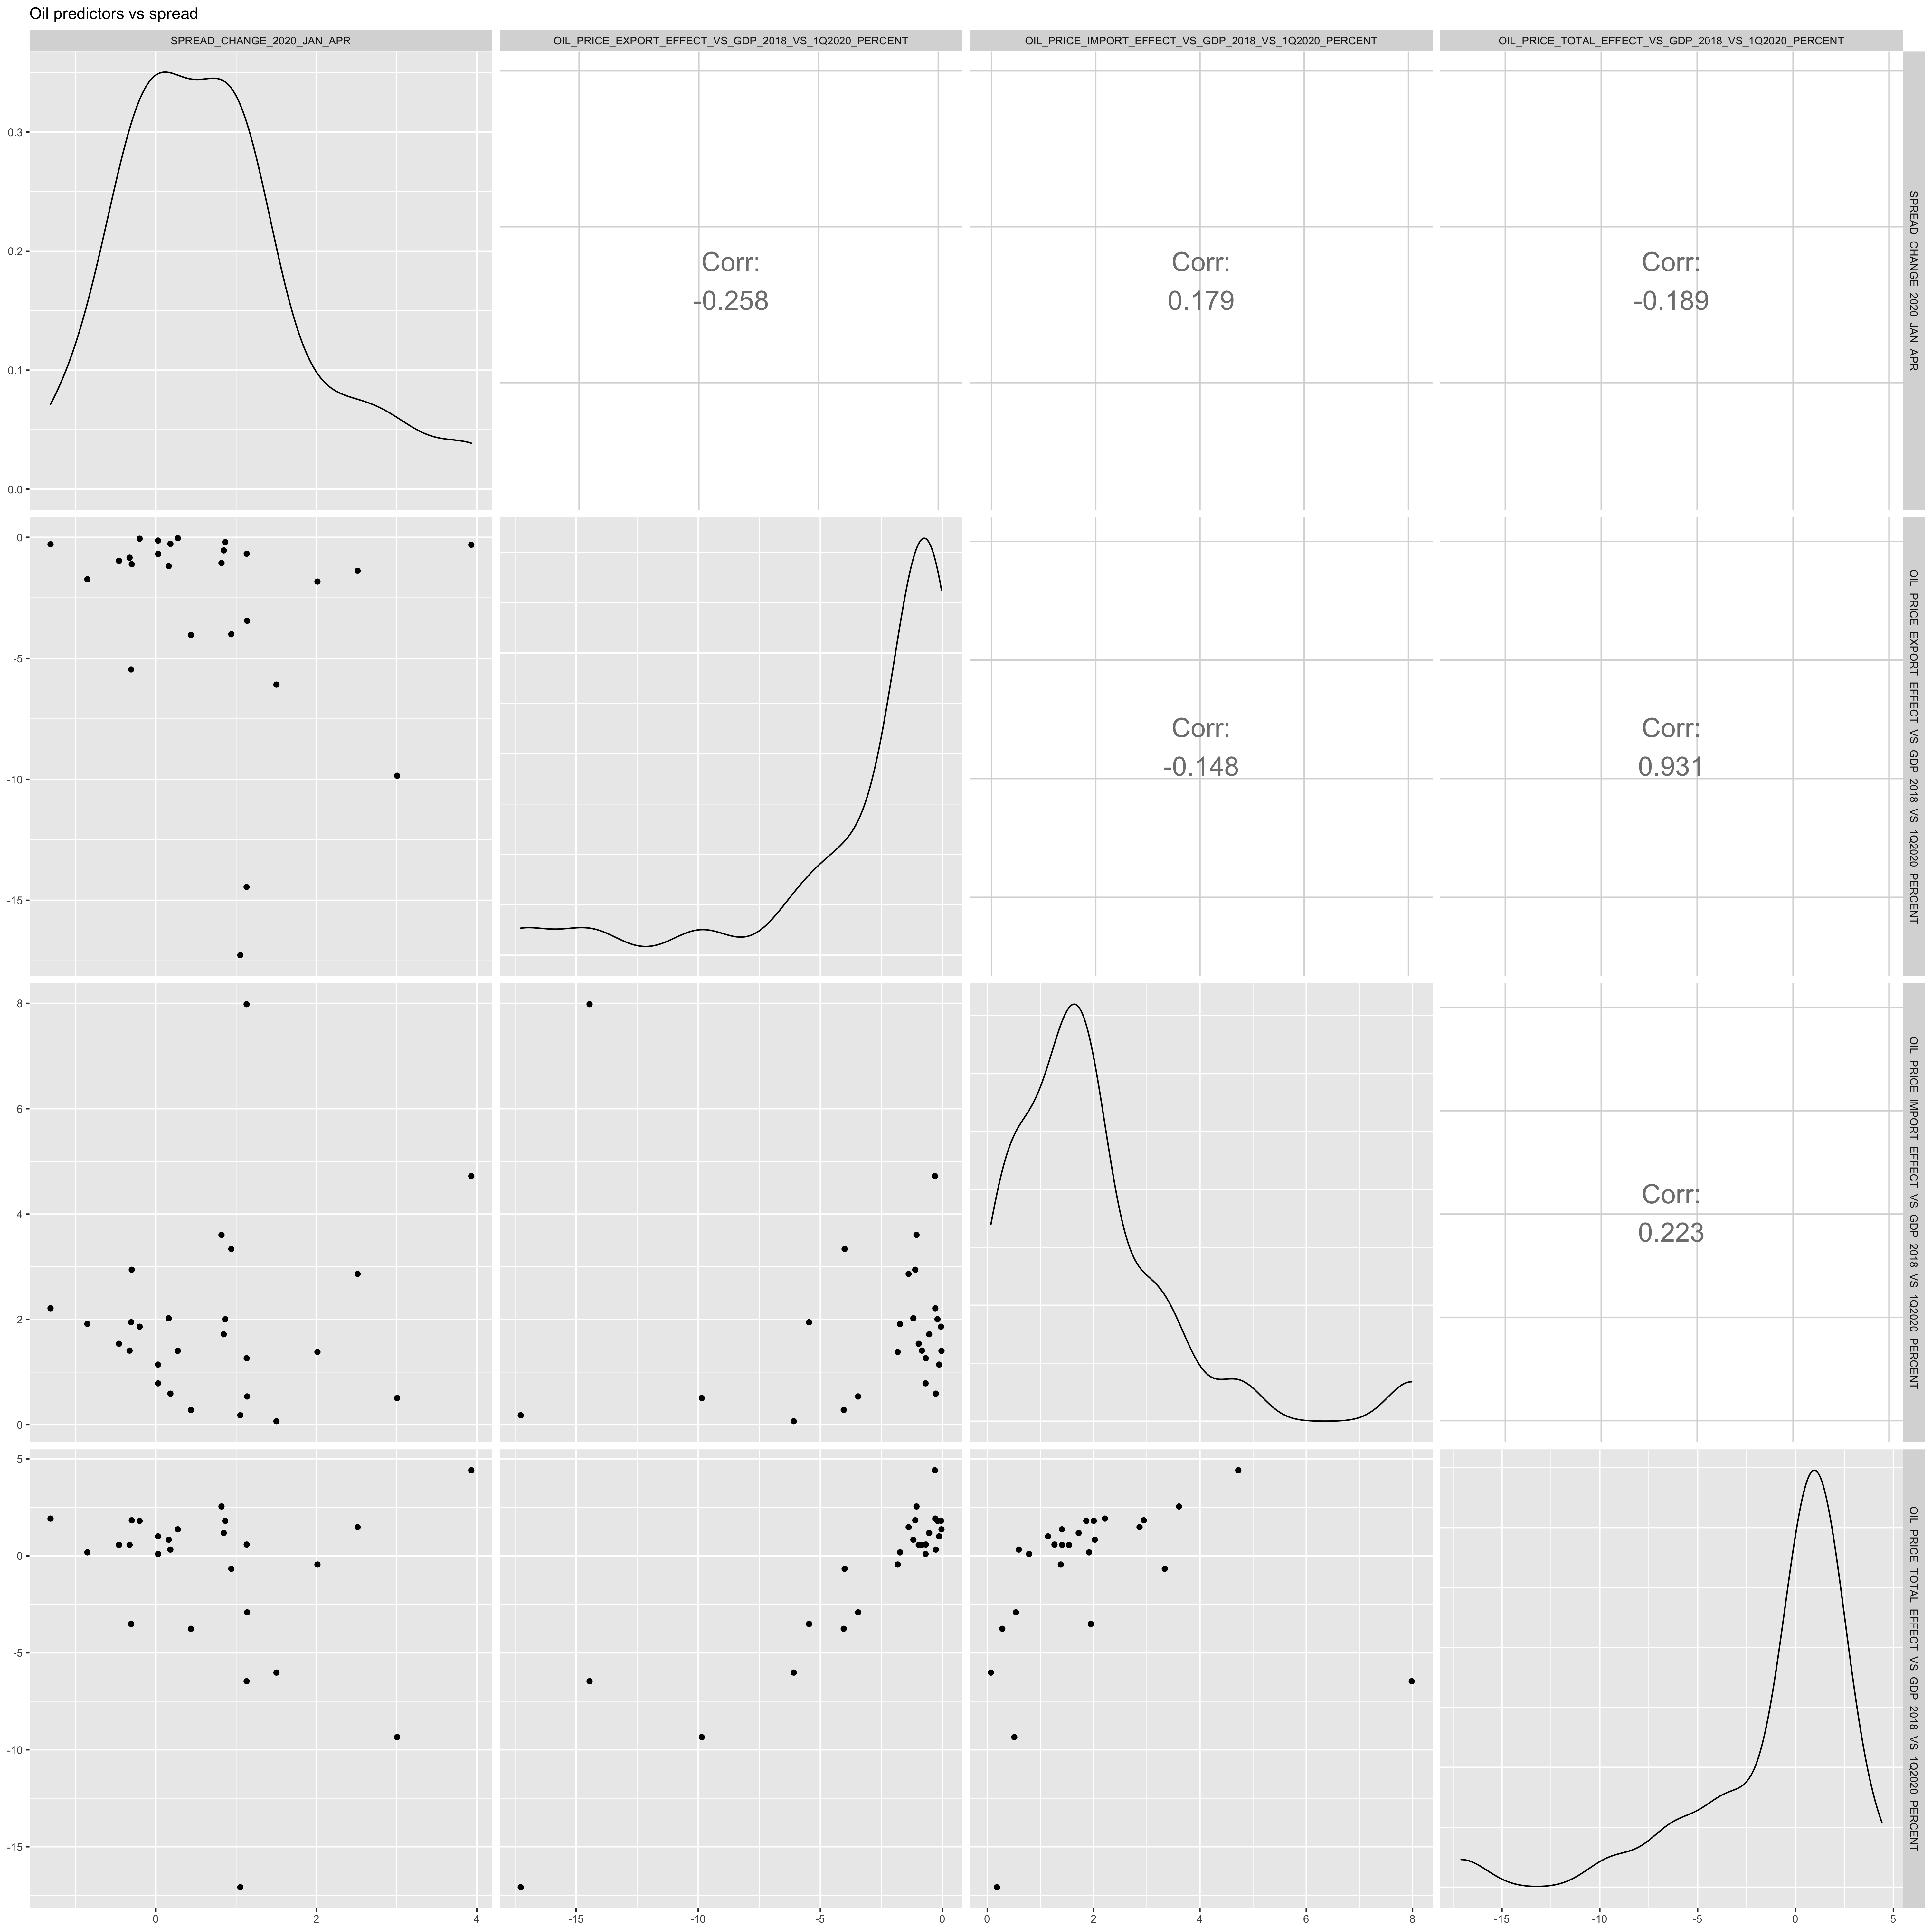
\includegraphics[width=0.5\textwidth,height=\textheight]{reportfigures/Corrmatrix_spread_vs_oil.png}
\caption{Correlation matrix of spread vs explantory variables from the
oil cluster}
\end{figure}

\hypertarget{correlation-heat-maps}{%
\subsection{Correlation heat maps}\label{correlation-heat-maps}}

\begin{figure}
\centering
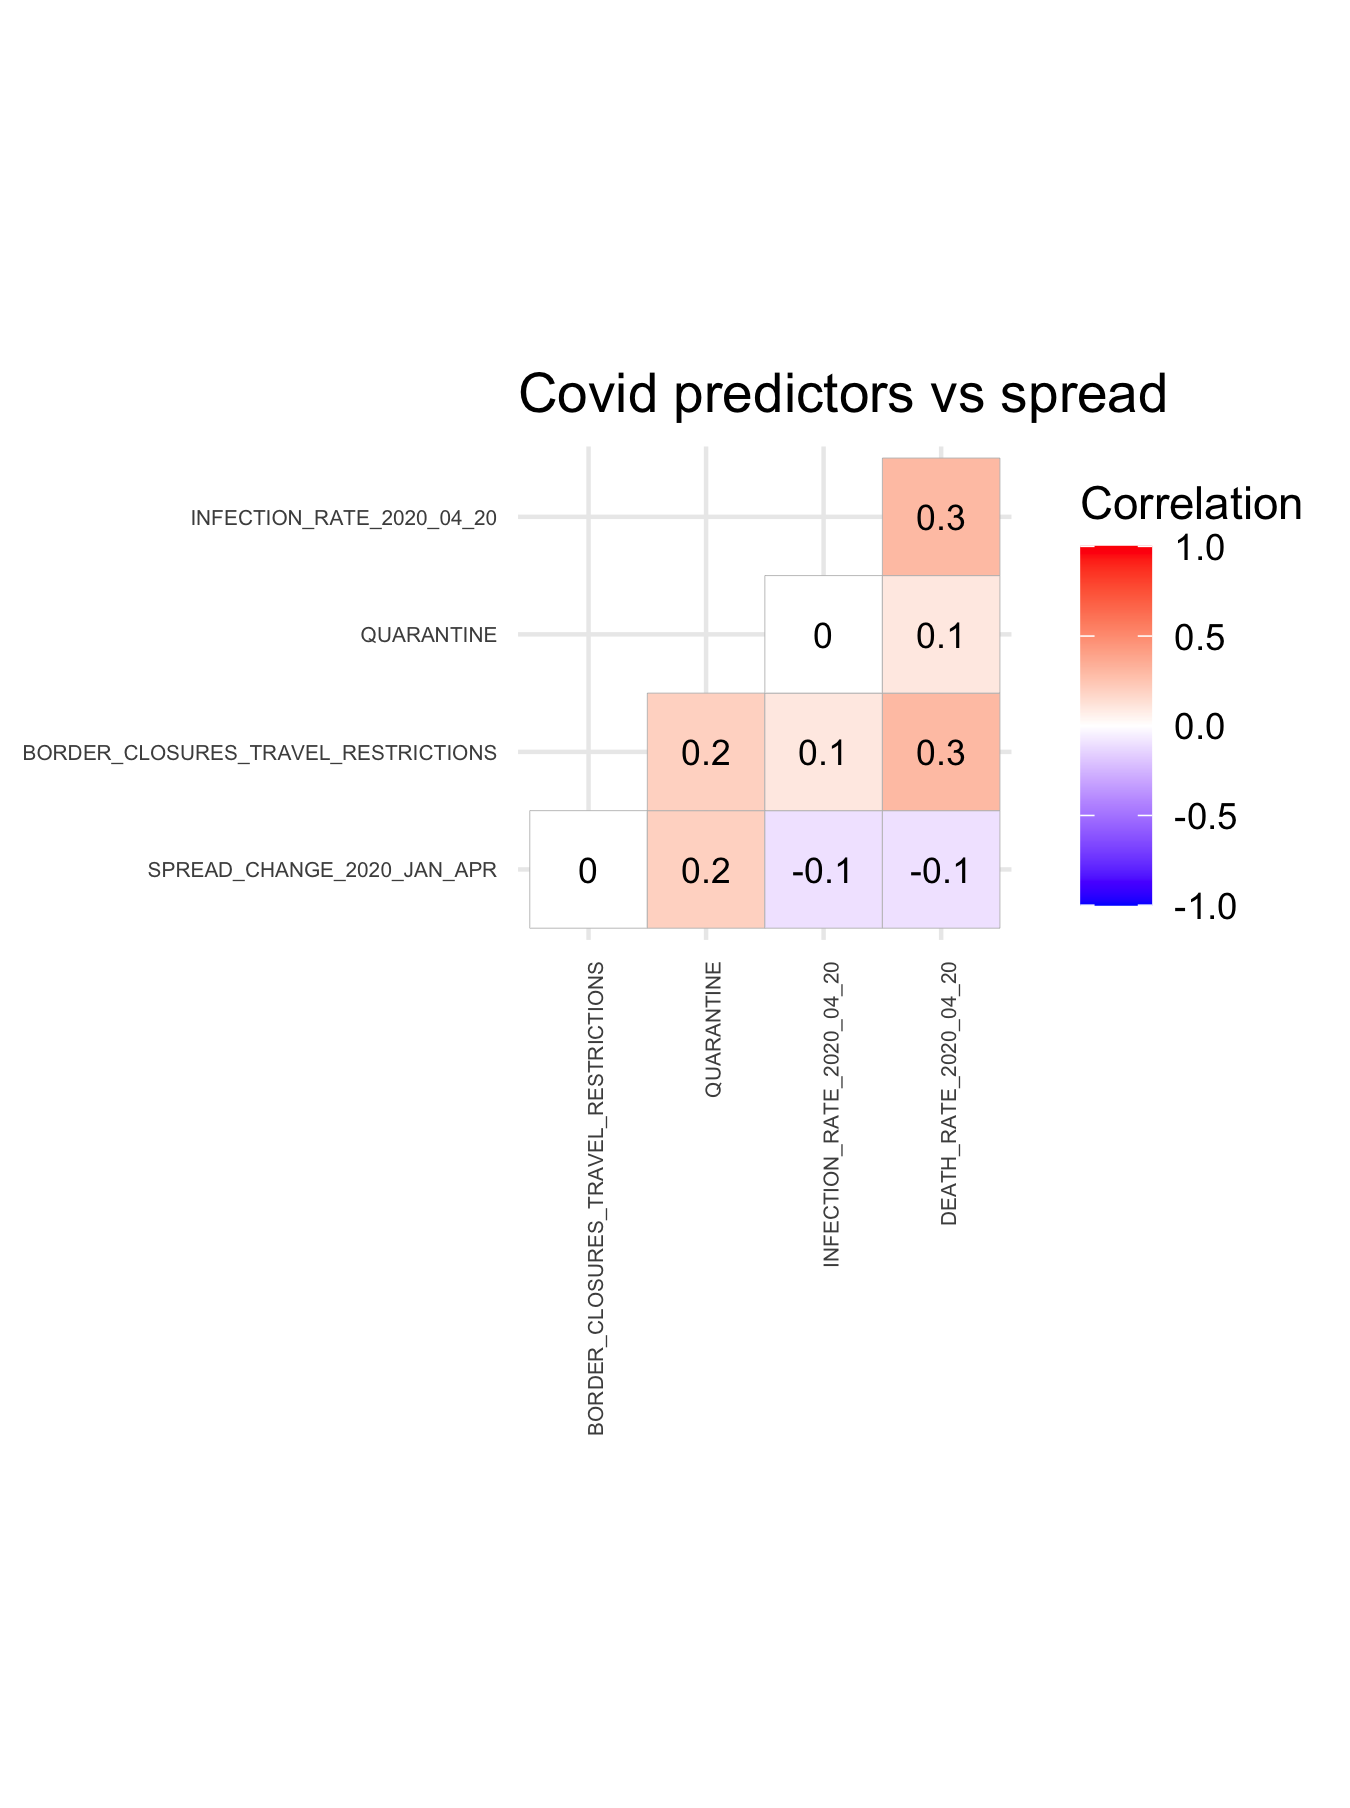
\includegraphics[width=0.5\textwidth,height=\textheight]{reportfigures/Corrplot_spread_vs_covid.png}
\caption{Correlation heatmap of spread vs explantory variables from the
epidemiologic cluster}
\end{figure}

\begin{figure}
\centering
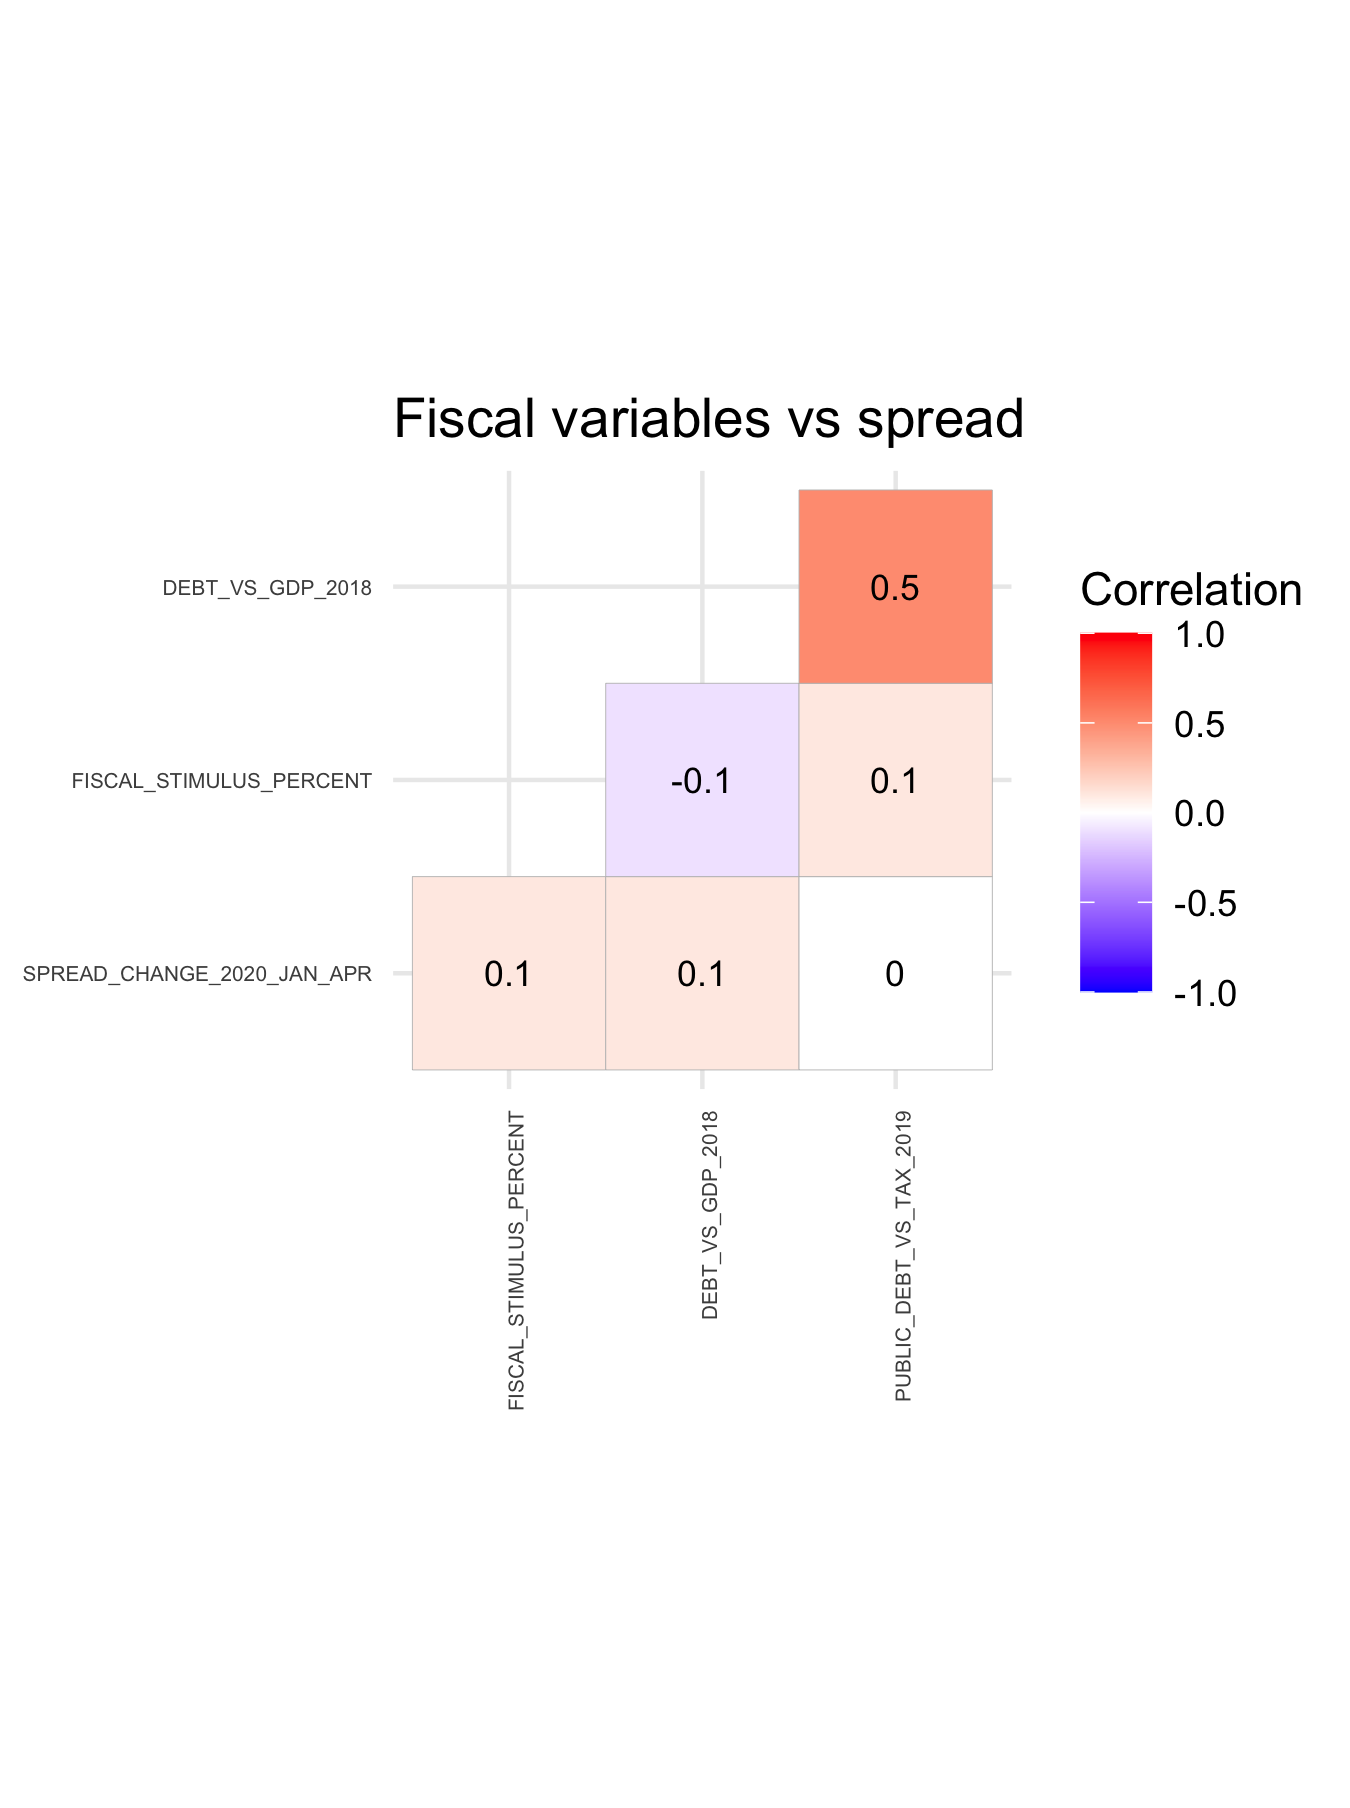
\includegraphics[width=0.5\textwidth,height=\textheight]{reportfigures/Corrplot_spread_vs_fiscal.png}
\caption{Correlation heatmap of spread vs explantory variables from the
fiscal cluster}
\end{figure}

\begin{figure}
\centering
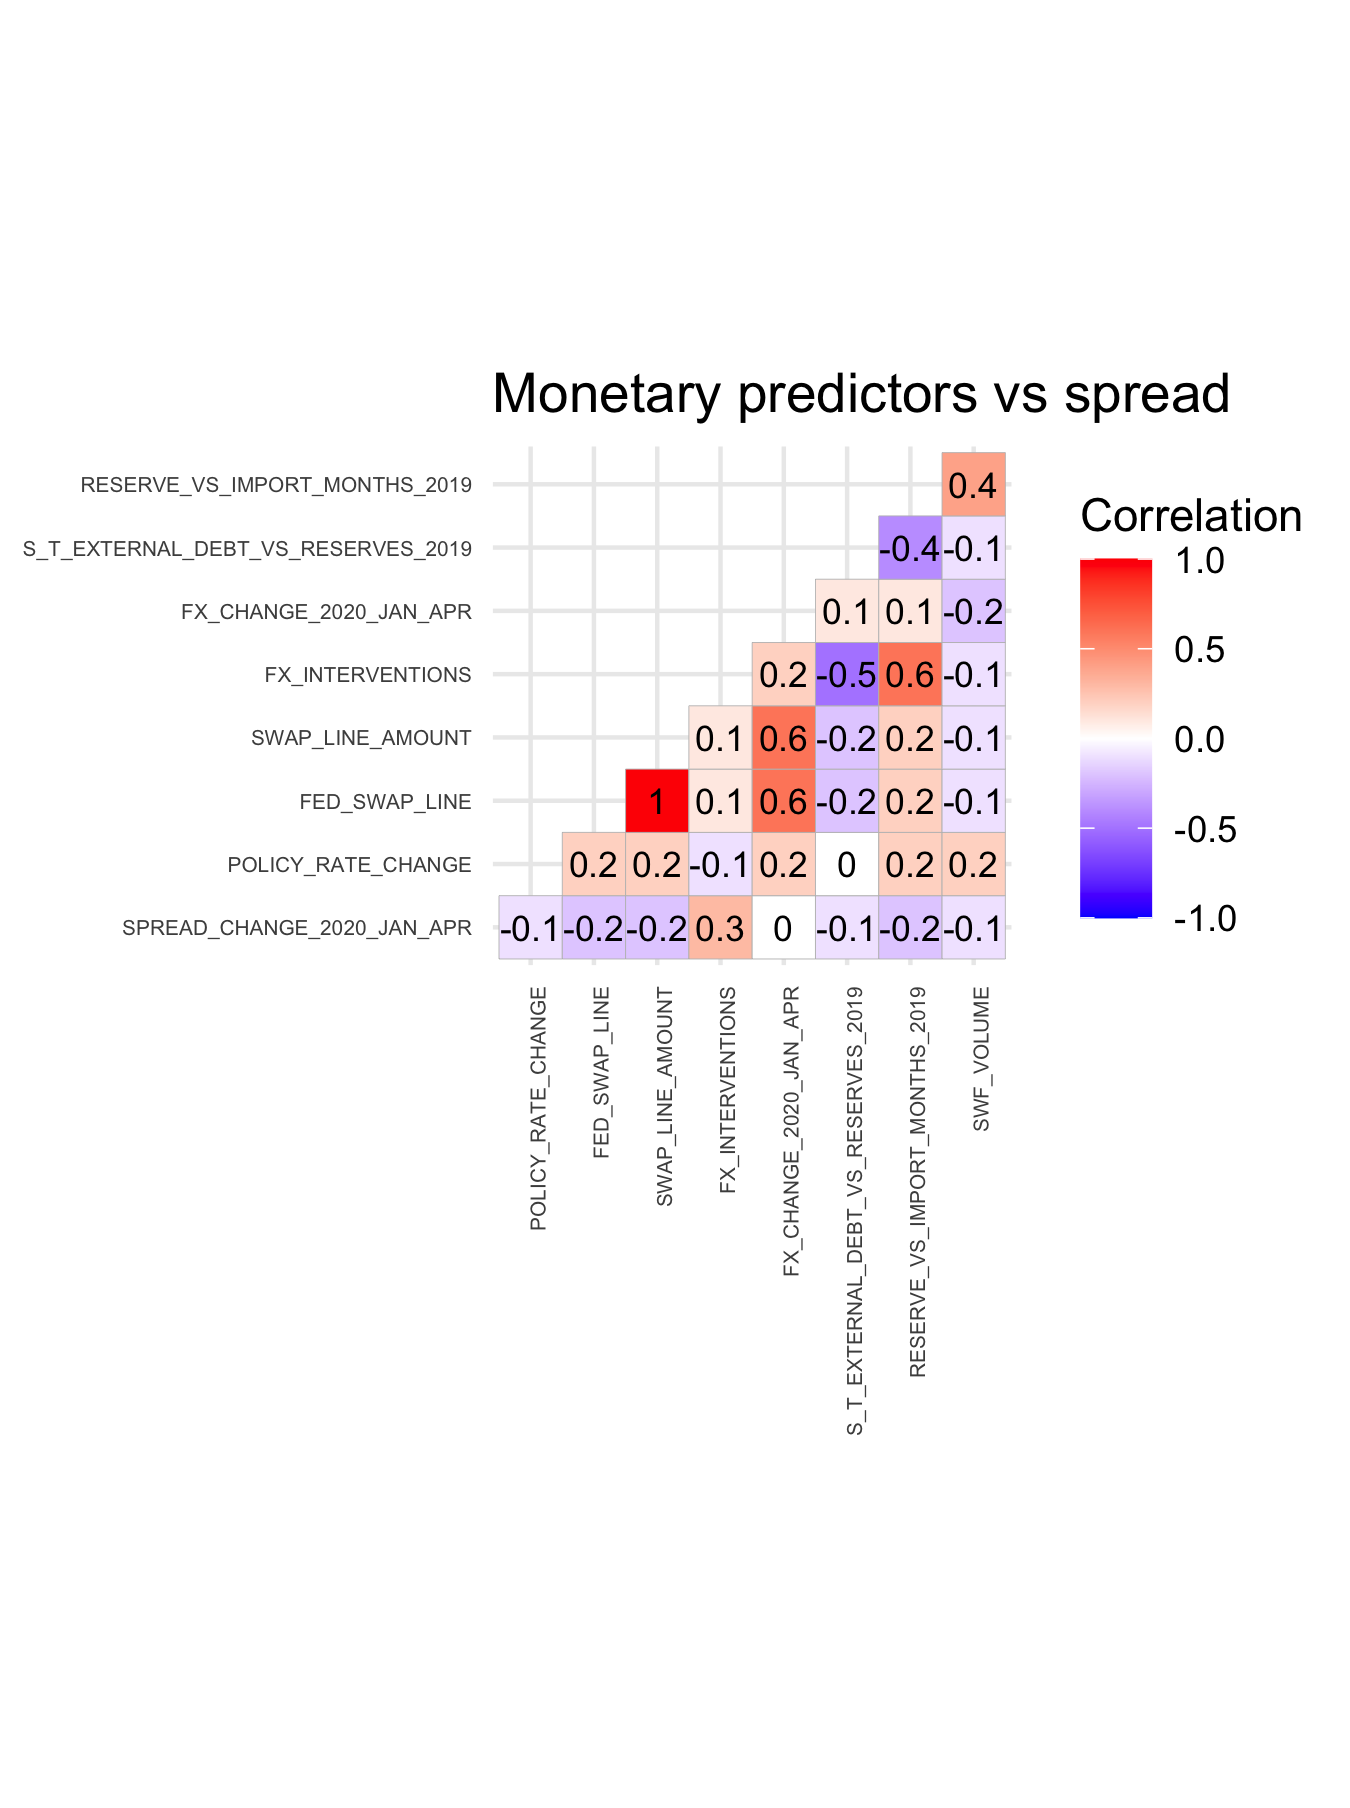
\includegraphics[width=0.5\textwidth,height=\textheight]{reportfigures/Corrplot_spread_vs_monetary.png}
\caption{Correlation heatmap of spread vs explantory variables from the
monetary cluster}
\end{figure}

\begin{figure}
\centering
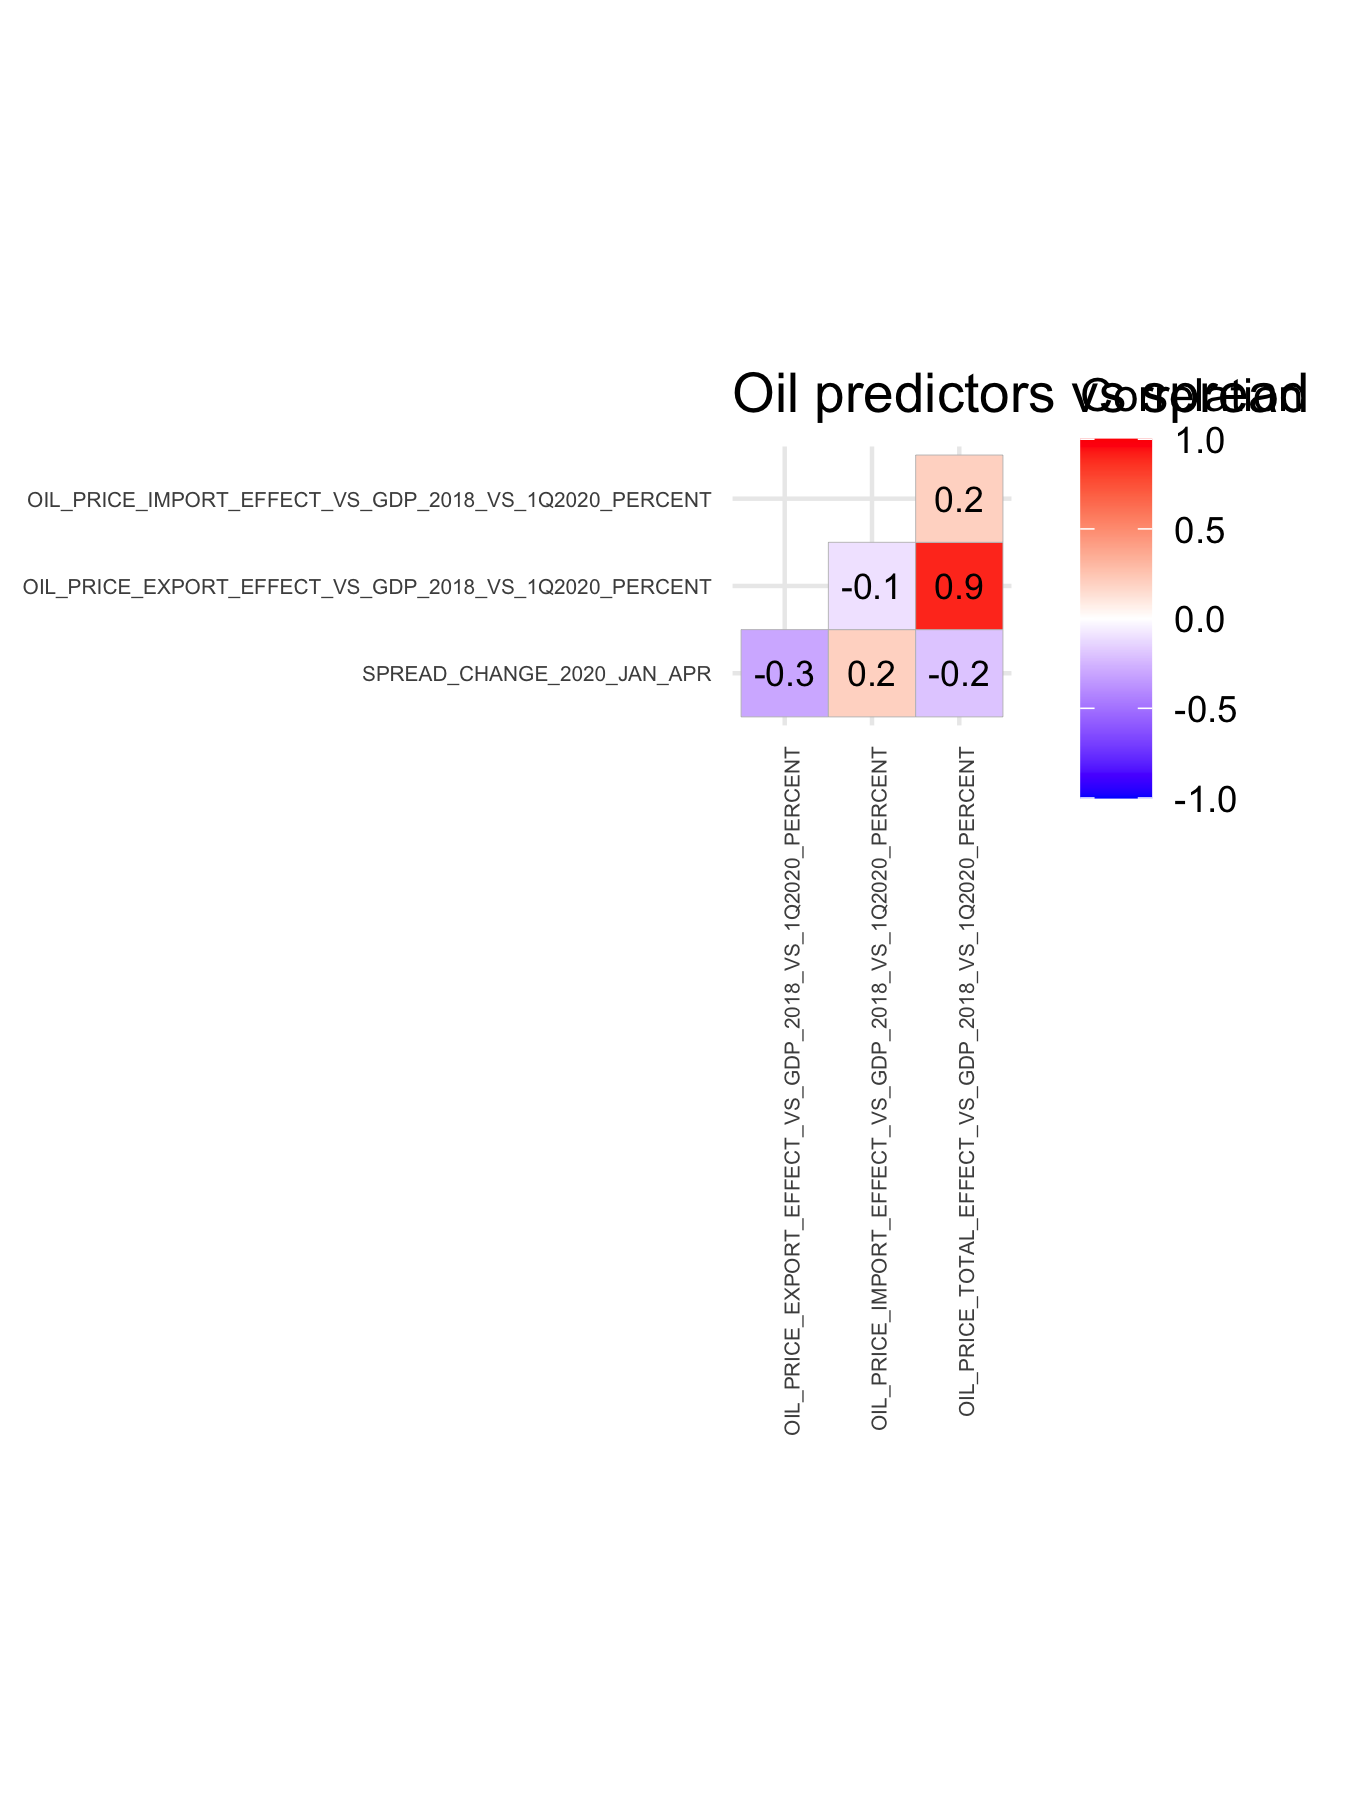
\includegraphics[width=0.5\textwidth,height=\textheight]{reportfigures/Corrplot_spread_vs_oil.png}
\caption{Correlation heatmap of spread vs explantory variables from the
oil cluster}
\end{figure}

\hypertarget{econometric-results}{%
\section{4. Econometric results}\label{econometric-results}}

\begin{figure}
\centering
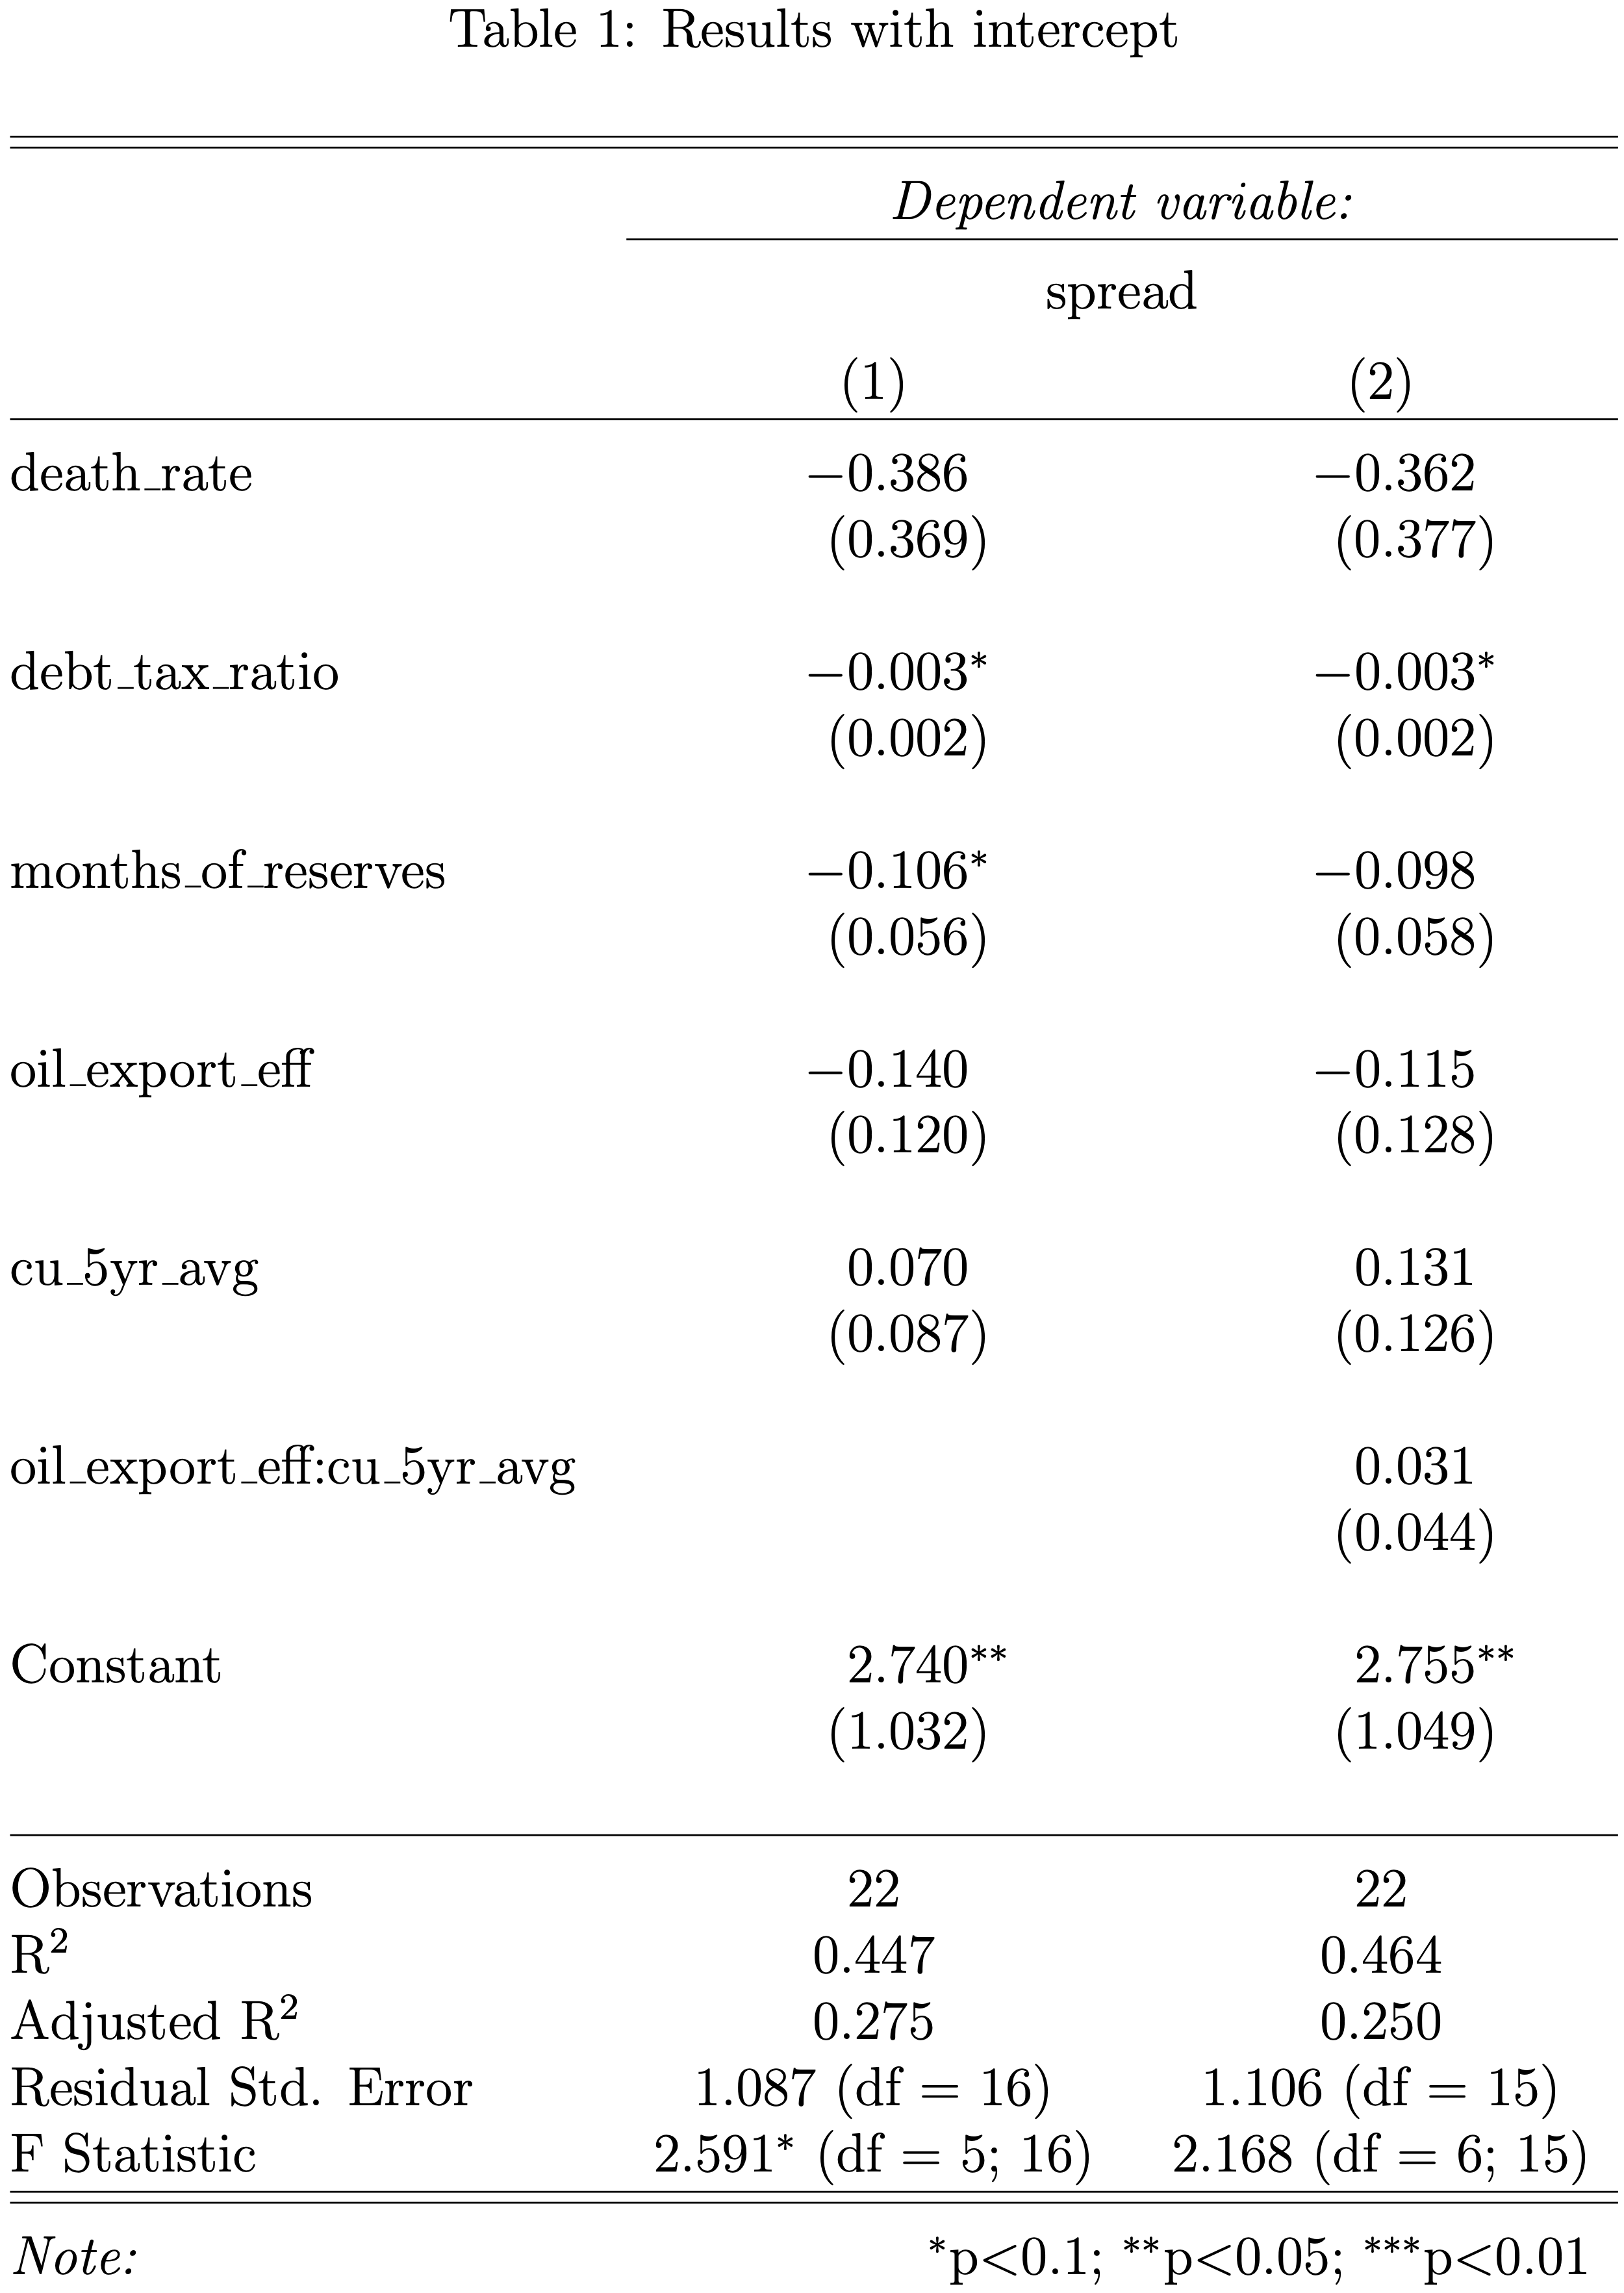
\includegraphics[width=0.5\textwidth,height=\textheight]{reportfigures/BEFORE_Regression__ouputs_when_using_debt_tax_ratio_intercept.png}
\caption{Regresson results using debt to tax ratio, with intercept}
\end{figure}

\begin{figure}
\centering
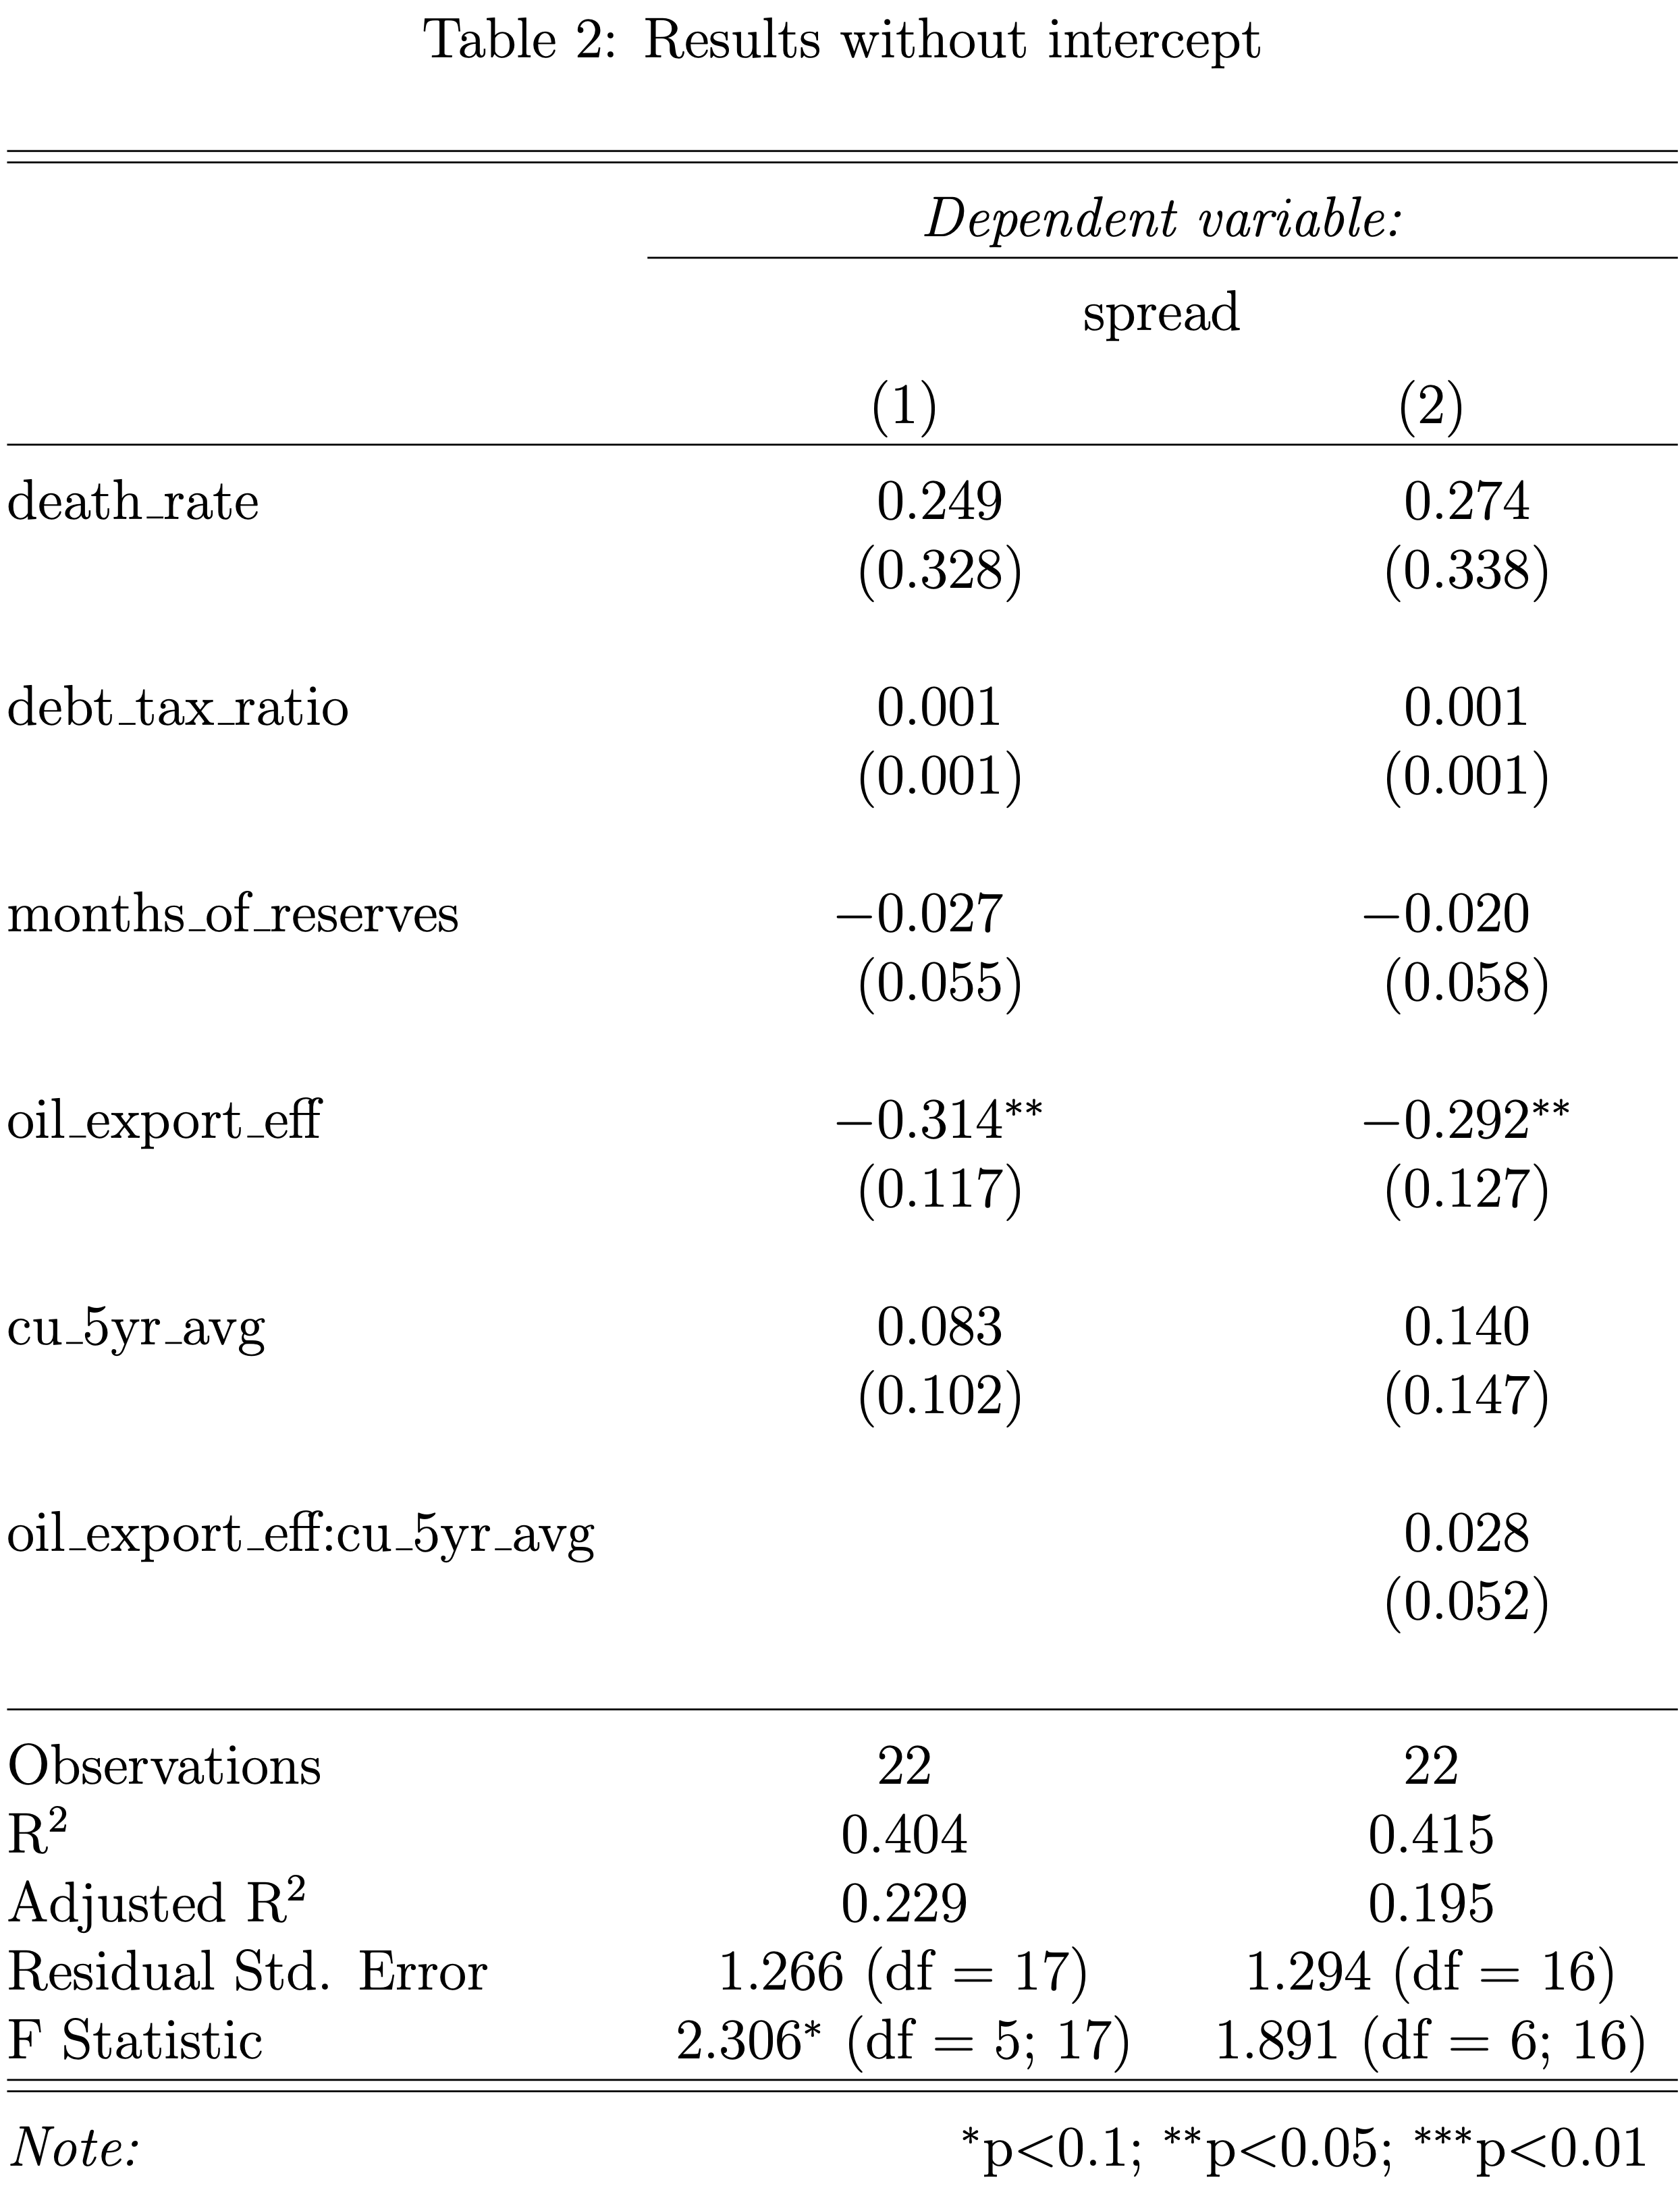
\includegraphics[width=0.5\textwidth,height=\textheight]{reportfigures/BEFORE_Regression__ouputs_when_using_debt_tax_ratio_nointercept.png}
\caption{Regresson results using debt to tax ratio, no intercept}
\end{figure}

\begin{figure}
\centering
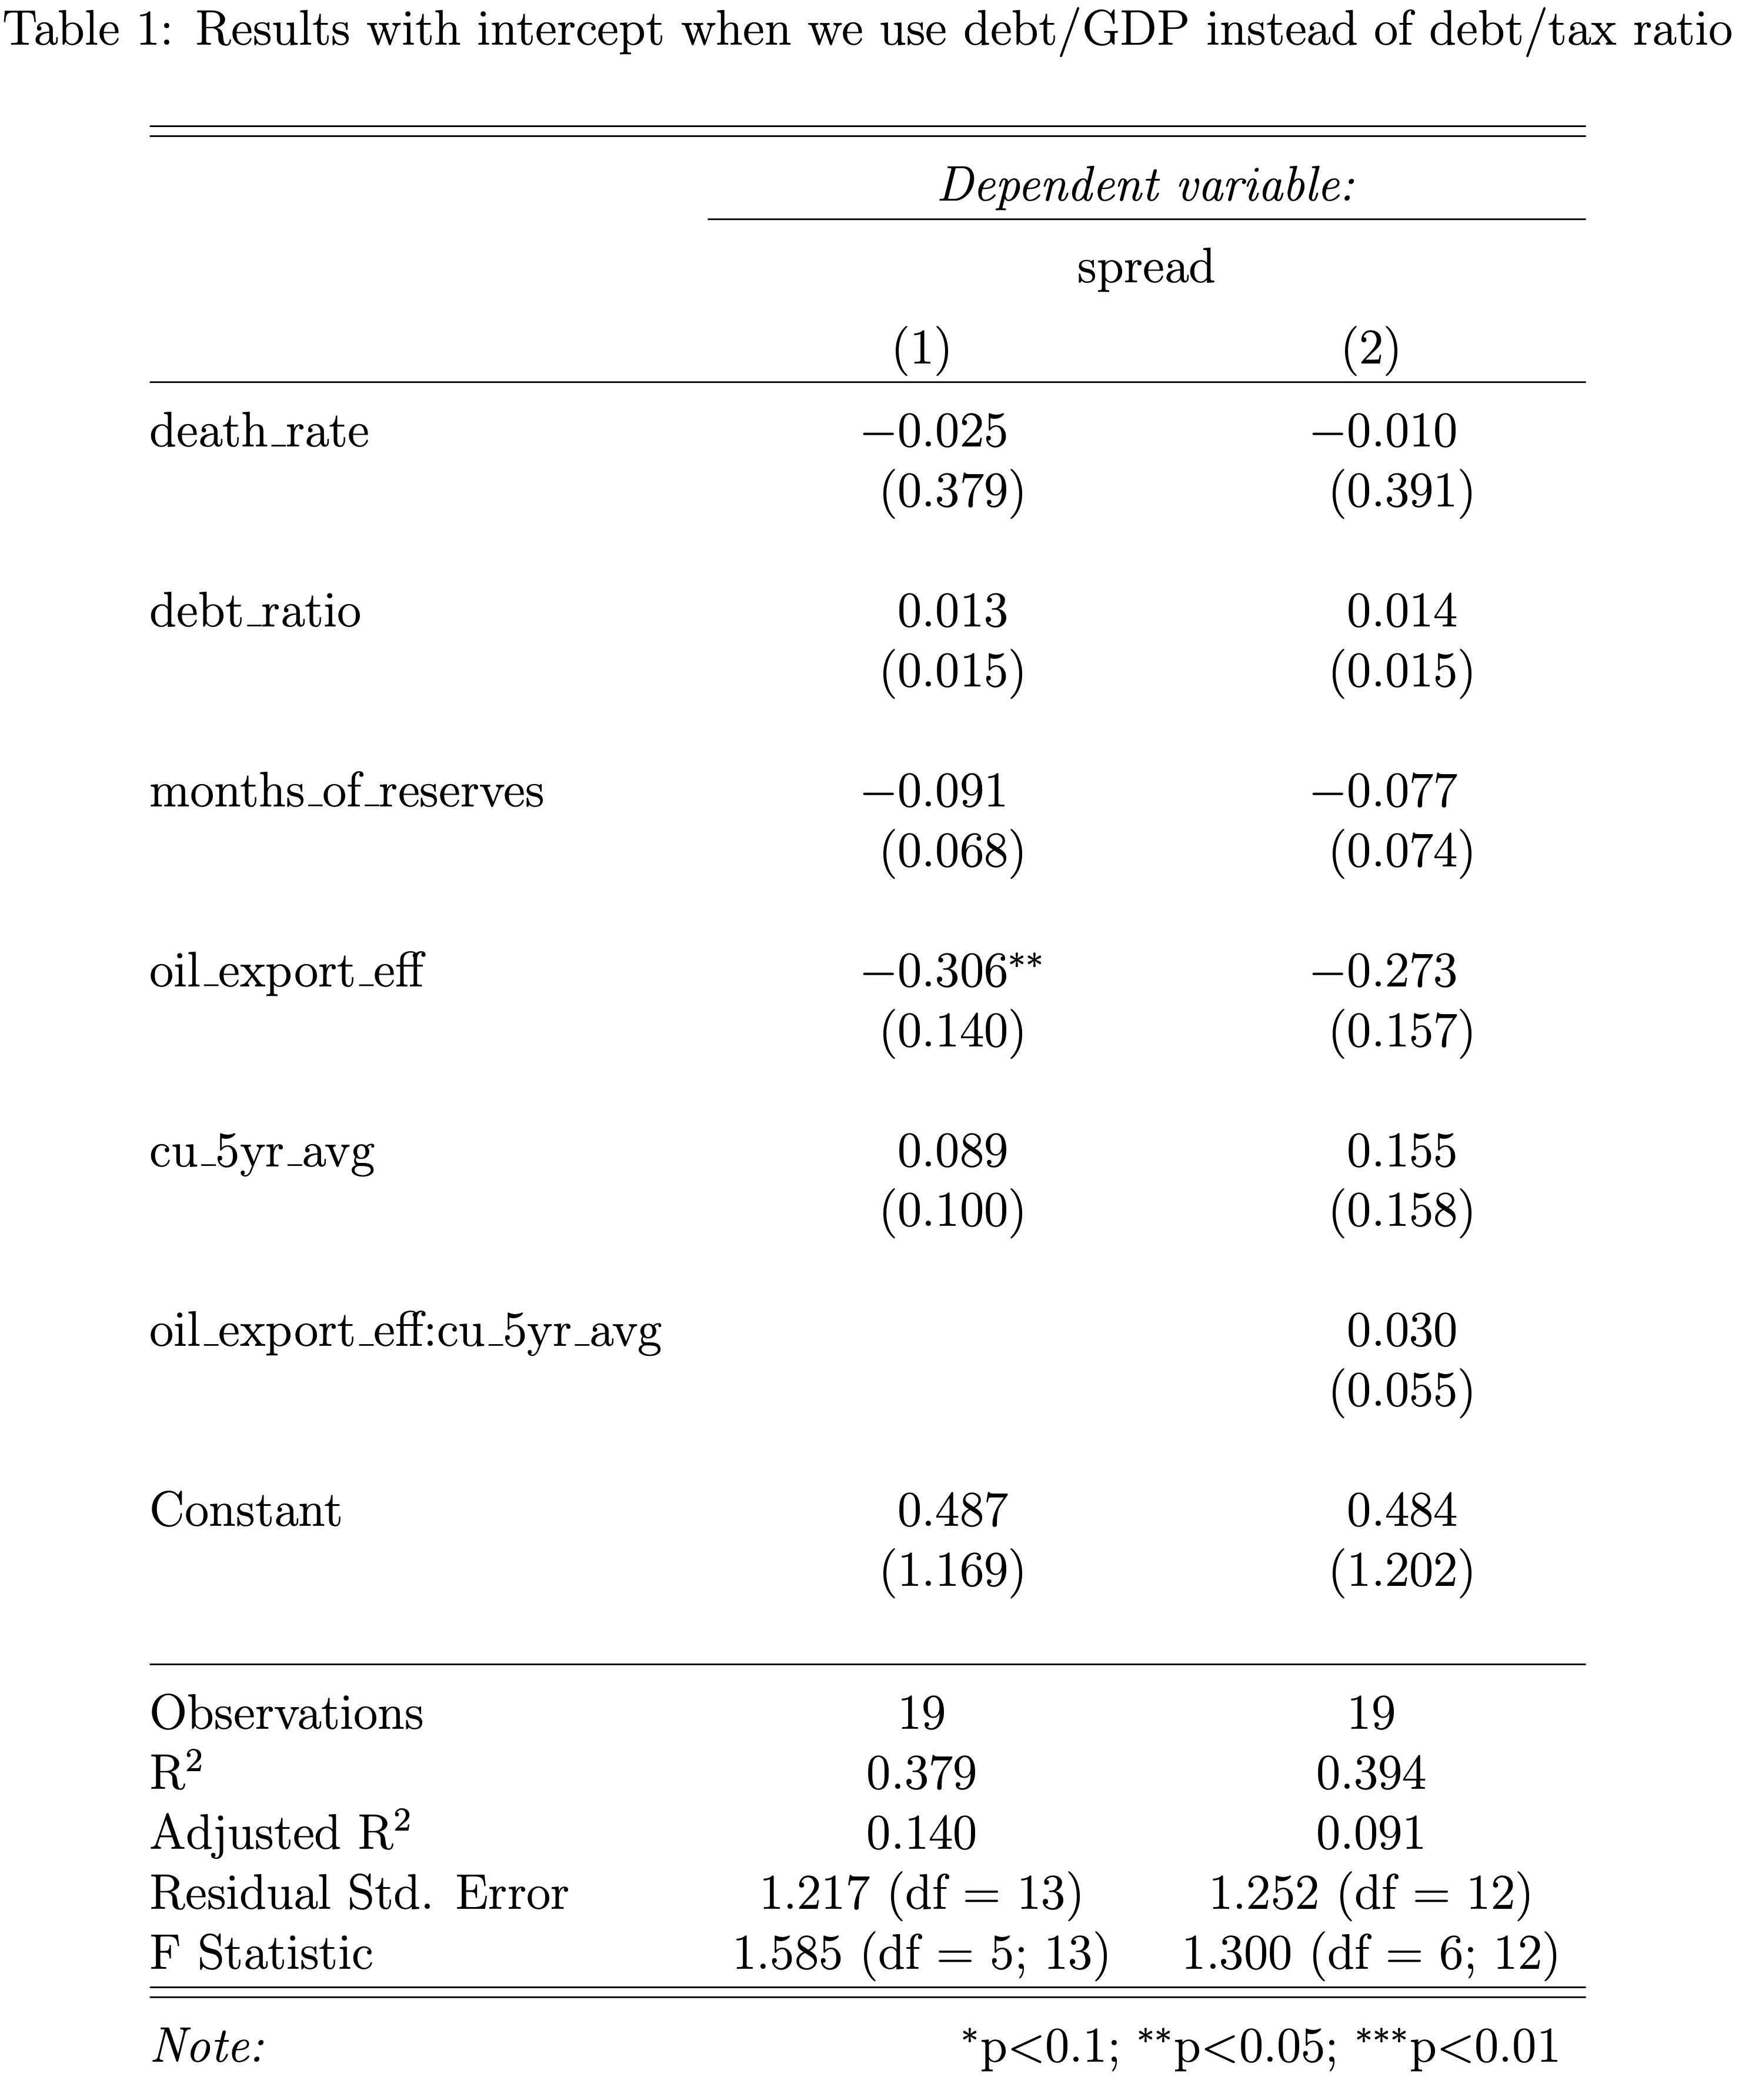
\includegraphics[width=0.5\textwidth,height=\textheight]{reportfigures/AFTER_Regression_outputs_when_using_debt_gdp_ratio_intercept.png}
\caption{Regresson results using debt gdp ratio, with intercept}
\end{figure}

\begin{figure}
\centering
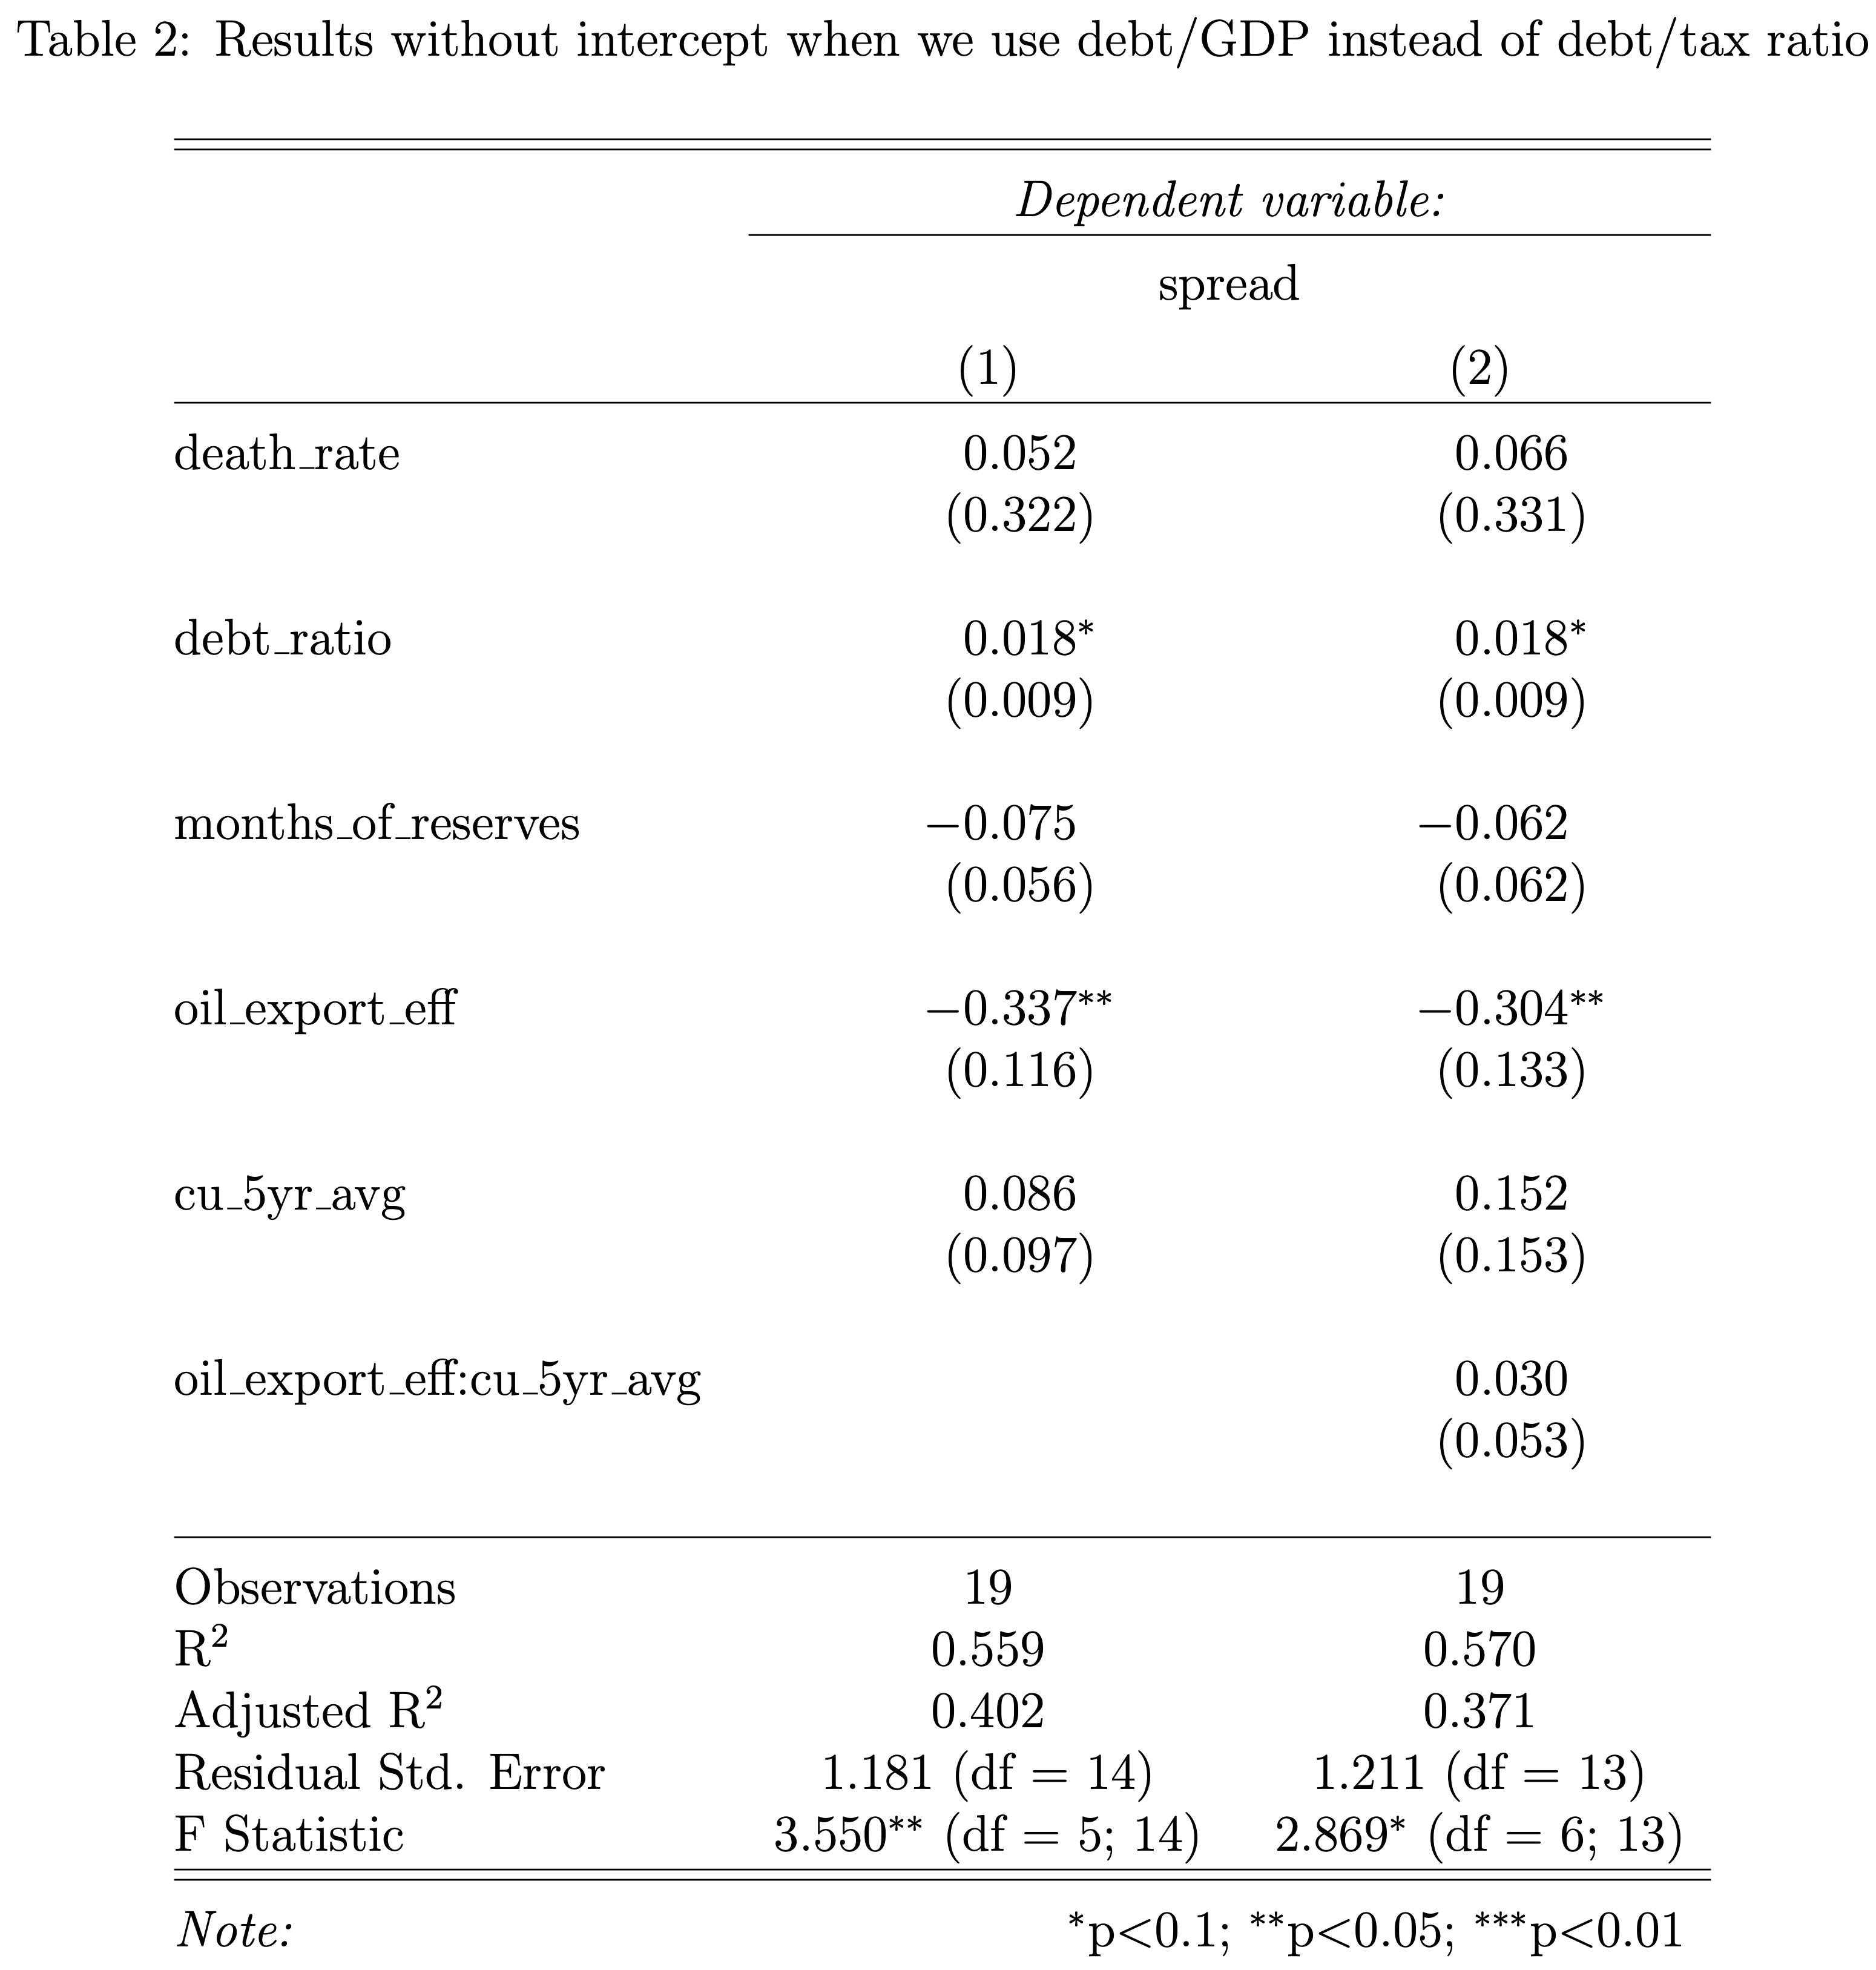
\includegraphics[width=0.5\textwidth,height=\textheight]{reportfigures/AFTER_Regression_outputs_when_using_debt_gdp_ratio_nointercept.png}
\caption{Regresson results using debt gdp ratio, no intercept}
\end{figure}

\hypertarget{conclusion}{%
\section{5. Conclusion}\label{conclusion}}

As stated in the introduction, this paper is preliminary. As more data
becomes available with the relase of June figures, the whole analysis
will be rerun to see if the results align more with theoretical
expectations or if there's potential variables that we have missed. It
may also be that there is a null-result: it is not clear at this point
in the pandemic which EM sovereigns will suffer the most. This may
actually not be an improbable result given that financial market
participants do not have a lot visibility and will probably stay on the
side line for all EM instead of being choosy.

\newpage
\singlespacing 
\bibliography{/Users/timodaehler/Desktop/COVID19DEBT/Text/Bibliography.bib}
\end{document}